\documentclass[11pt]{article}
% =====================================================================
%  ARCHIVED VERSION 1 -- standalone Study-1-only paper (pre-CHI-restructure).
%  Kept for provenance/rollback. The current paper is main.tex (3-study CHI).
%  Compile:  latexmk -pdf main_study1_only.tex
% =====================================================================
\usepackage[utf8]{inputenc}
\usepackage[T1]{fontenc}
\usepackage[margin=1in]{geometry}
\usepackage{graphicx}
\graphicspath{{../figures/}}
\usepackage[table,dvipsnames]{xcolor}
\usepackage{booktabs}
\usepackage{longtable}
\usepackage{array}
\usepackage{amsmath,amssymb}
\usepackage{caption}
\usepackage{subcaption}
\usepackage{enumitem}
\usepackage{microtype}
\usepackage[numbers,sort&compress]{natbib}
\usepackage[colorlinks=true,linkcolor=NavyBlue,citecolor=BrickRed,urlcolor=NavyBlue]{hyperref}
\usepackage{titlesec}

\definecolor{g}{RGB}{26,152,80}
\definecolor{a}{RGB}{254,224,139}
\definecolor{r}{RGB}{215,48,39}

% auto-generated - do not edit by hand (see analysis/make_figures.py)
\newcommand{\Nstudies}{217}
\newcommand{\Ndomains}{29}
\newcommand{\Nvalidated}{8}
\newcommand{\Npromising}{60}
\newcommand{\Nmixed}{108}
\newcommand{\Ncaution}{39}
\newcommand{\Nunreliable}{2}
\newcommand{\Pctreliable}{31}
\newcommand{\Pctproblematic}{19}
\newcommand{\Nnumeric}{29}
\newcommand{\Nprimary}{206}
\newcommand{\Nsecondary}{11}
\newcommand{\Ngreen}{8}
\newcommand{\Namber}{19}
\newcommand{\Nred}{2}
\newcommand{\OAretrieved}{1500}
\newcommand{\OAunique}{957}
\newcommand{\OAtopical}{165}
\newcommand{\Webhits}{472}
\newcommand{\Webunique}{304}
\newcommand{\Nassessed}{263}
\newcommand{\Nexclscreen}{967}
\newcommand{\Crossdup}{31}
\newcommand{\Meanrel}{3.15}
\newcommand{\Nparity}{15}


\titleformat{\section}{\large\bfseries}{\thesection}{0.6em}{}
\titleformat{\subsection}{\normalsize\bfseries}{\thesubsection}{0.6em}{}

\title{\textbf{When Can a Machine Judge Like a Human?}\\[2pt]
\large A PRISMA Systematic Review of LLM-as-a-Judge versus Human Annotation\\
across \Ndomains{} Domains and Tasks}
\author{Carlos Toxtli\thanks{Correspondence: \texttt{ai4helab@gmail.com}. AI-assisted systematic-search and
extraction pipeline; all search logs, the extracted-studies dataset, the analysis code, and the figure-generation
scripts are released for reproducibility.}}
\date{May 2026}

\begin{document}
\maketitle

\begin{abstract}
\noindent
Large language models (LLMs) are increasingly deployed as automatic \emph{judges} and \emph{annotators}. Adoption
has outpaced validation, and the field lacks a panoramic answer to the question that matters: \emph{not} ``do LLM
judges work?'' but ``\emph{in which domains, tasks, and conditions} do LLM judgments agree with human judgments well
enough to substitute for them?'' We address this with a PRISMA~2020 systematic review. Using a triangulated
identification strategy---OpenAlex (\OAretrieved{} records, \OAunique{} unique), Semantic Scholar, and a web
deep-search---we screened \Nexclscreen{}+ records and included \Nstudies{} studies across \Ndomains{} domains. Each
was coded on a five-level reliability rubric benchmarked against the \emph{human--human} ceiling. Only \Pctreliable\%
of studies place LLM judges at or near validated substitution; the modal verdict is \emph{mixed/task-dependent}
(mean reliability \Meanrel/5). Reliability is high---often exceeding the human ceiling---for objective,
well-structured, low-expertise tasks judged at the aggregate level, and collapses for subjective, expert,
low-resource, or adversarial settings. We provide a domain$\times$task reliability landscape, a deployment decision
map, a catalogue of failure modes, and a validation checklist.
\end{abstract}

\tableofcontents
\bigskip

\section{Introduction}
The cost, latency, and irreproducibility of human evaluation have made ``LLM-as-a-judge'' the dominant scalable
surrogate \citep{zheng2023mtbench,gu2024survey}. Yet a model that matches human preferences at $>$80\% on chat
\citep{zheng2023mtbench} can correlate near zero with expert creativity judgments \citep{chakrabarty2024artartifice},
or be fooled into mislabeling relevance by a few injected keywords \citep{alaofi2024fooledrelevant}. This review maps,
domain by domain and task by task, the conditions under which LLM--human agreement is good enough to substitute,
anchoring every claim to the human--human ceiling. Contributions: a PRISMA review of \Nstudies{} studies across
\Ndomains{} domains; a reproducible five-level reliability rubric; a reliability landscape and decision map; and
synthesis along the judge-architecture axis.

\section{Background and related reviews}
LLM-as-a-judge descends from reference-free metrics but uses a general instruction-following model with a
natural-language rubric \citep{li2024compsurvey,gao2025nlgsurvey}. Four architectural families recur: prompted
general LLMs \citep{zheng2023mtbench,liu2023geval}; fine-tuned open evaluators \citep{kim2023prometheus,
zhu2023judgelm,wang2023pandalm,li2023autoj,wang2023shepherd}; juries/multi-agent panels \citep{verga2024poll,
chan2023chateval}; and calibrated rubric methods \citep{hashemi2024llmrubric,fan2024sedareval}. Prior surveys
taxonomize methodology \citep{gu2024survey,li2024gen2judge}; large meta-evaluations supply task-level data
\citep{bavaresco2024judgebench,tan2024judgebench,calderon2025alttest,judgesverdict2025}. This review synthesizes the
cross-domain reliability map they imply.

\section{Methods}\label{sec:rubric}
We followed PRISMA~2020 \citep{page2021prisma}. \textbf{Inclusion:} empirical studies (2023--2026) that directly
compare LLM judgments to human judgments and report an agreement metric or structured concordance. Identification
triangulated OpenAlex (primary; \OAretrieved{} retrieved, \OAunique{} unique), Semantic Scholar, and a 59-query web
search (Figure~\ref{fig:prisma}). Each study was coded for domain, task formulation, subjectivity, expertise, judge
model/architecture, comparator, metric, headline agreement, human baseline, biases, and a five-level reliability
verdict (1 Validated $\dots$ 5 Unreliable) benchmarked against the human ceiling; reliability score $=6-$verdict.

\begin{figure}[t]\centering
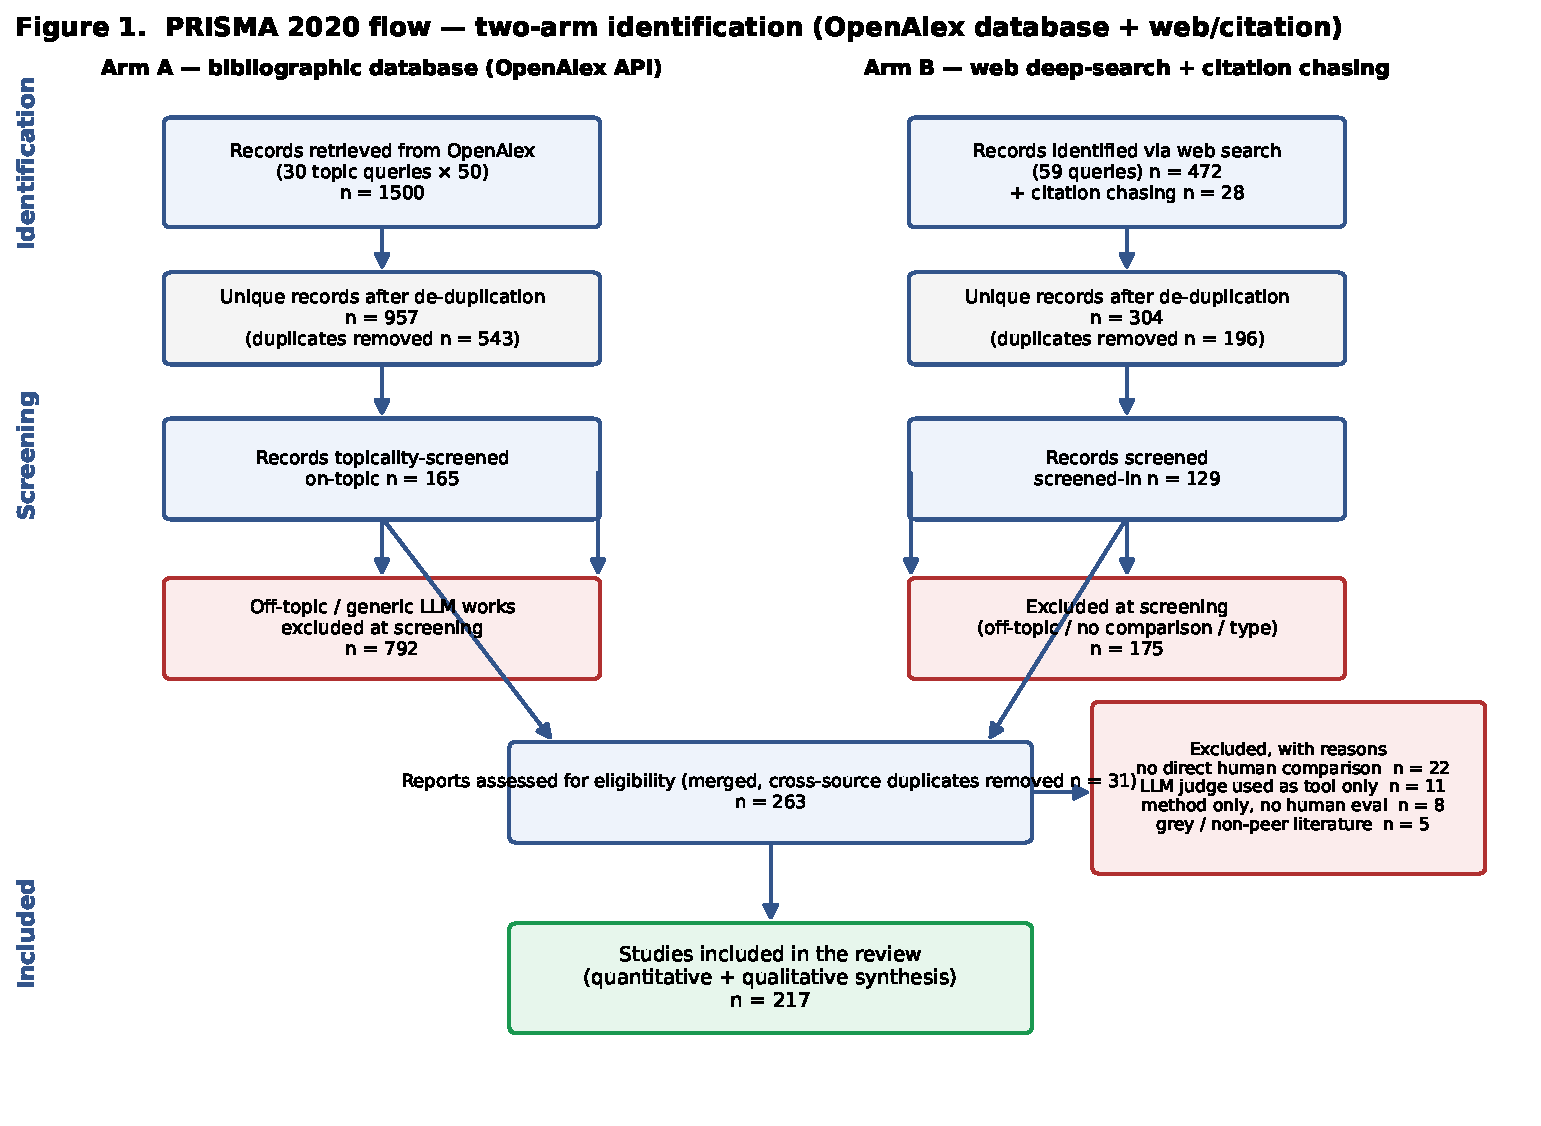
\includegraphics[width=\linewidth]{fig01_prisma_flow}
\caption{PRISMA~2020 two-arm identification (OpenAlex database + web/citation).}\label{fig:prisma}
\end{figure}

\section{Results}
\subsection{Corpus overview}
The \Nstudies{} studies span \Ndomains{} domains (Figure~\ref{fig:coverage}), concentrated in methodology/bias,
general NLG, education, medicine, and social-science annotation; by venue the corpus is ML/NLP-dominant with HCI/CSCW
and domain-journal representation. Volume rises across 2023--2026 (Figure~\ref{fig:year}); the objective/mixed/
subjective split (Figure~\ref{fig:method}) is the strongest predictor of reliability.

\begin{figure}[t]\centering
\begin{subfigure}{0.49\linewidth}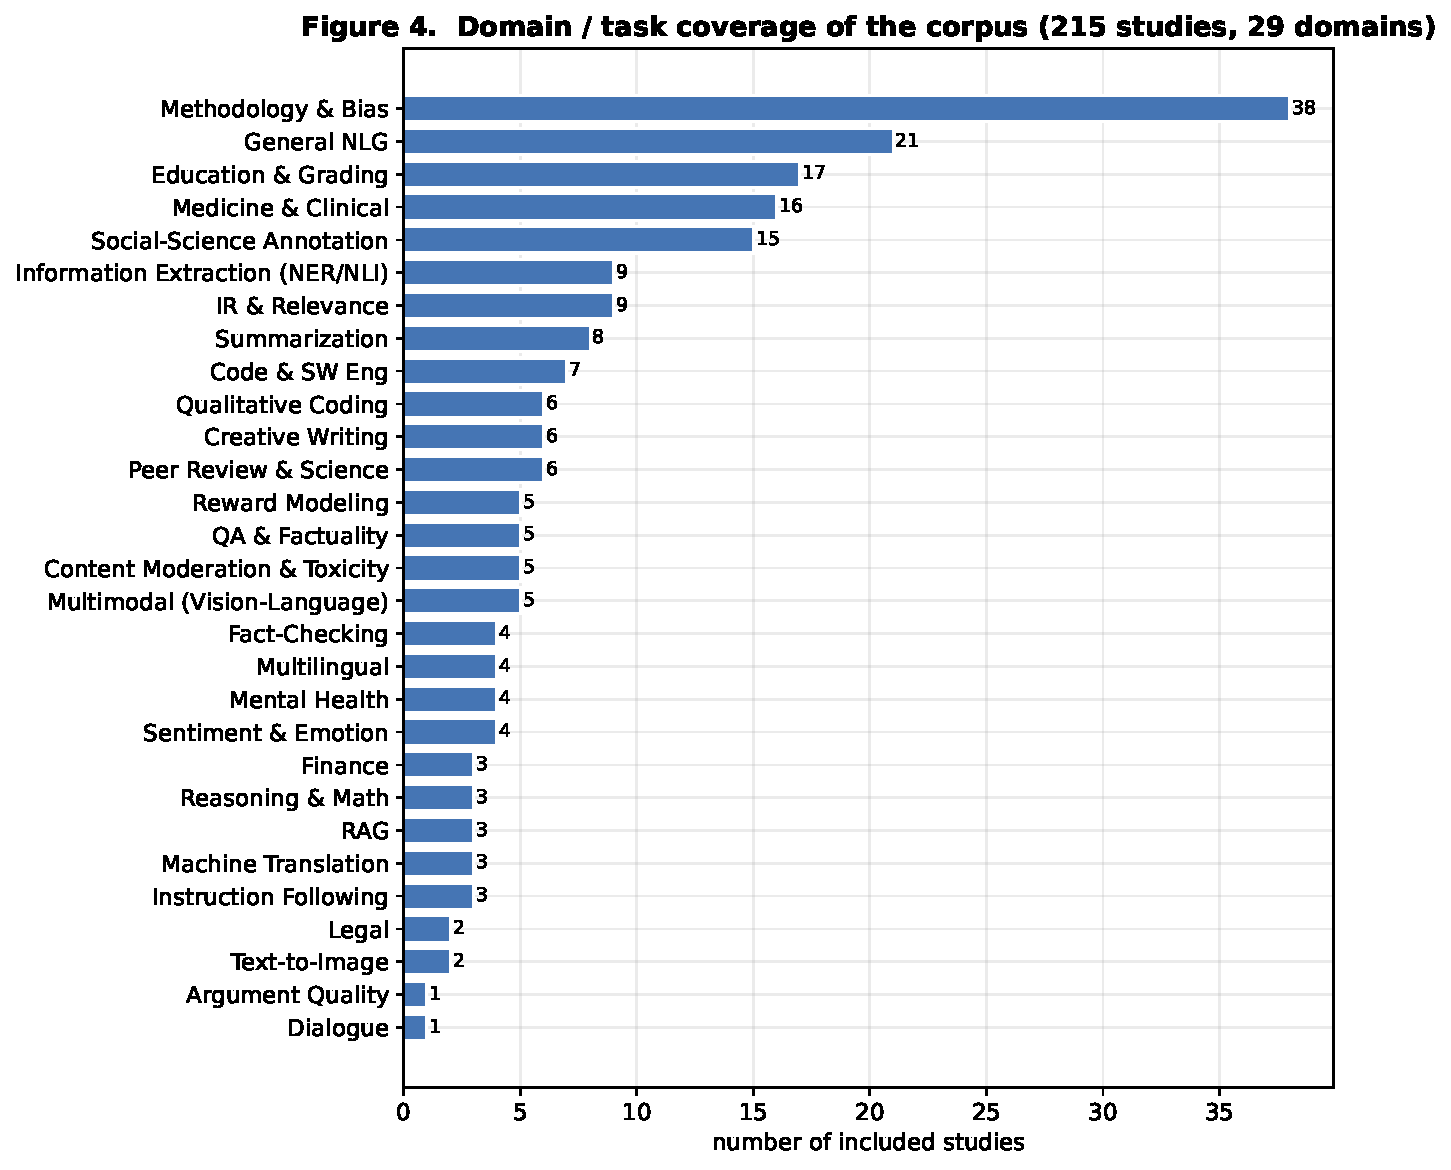
\includegraphics[width=\linewidth]{fig04_domain_counts}\caption{}\label{fig:coverage}\end{subfigure}\hfill
\begin{subfigure}{0.49\linewidth}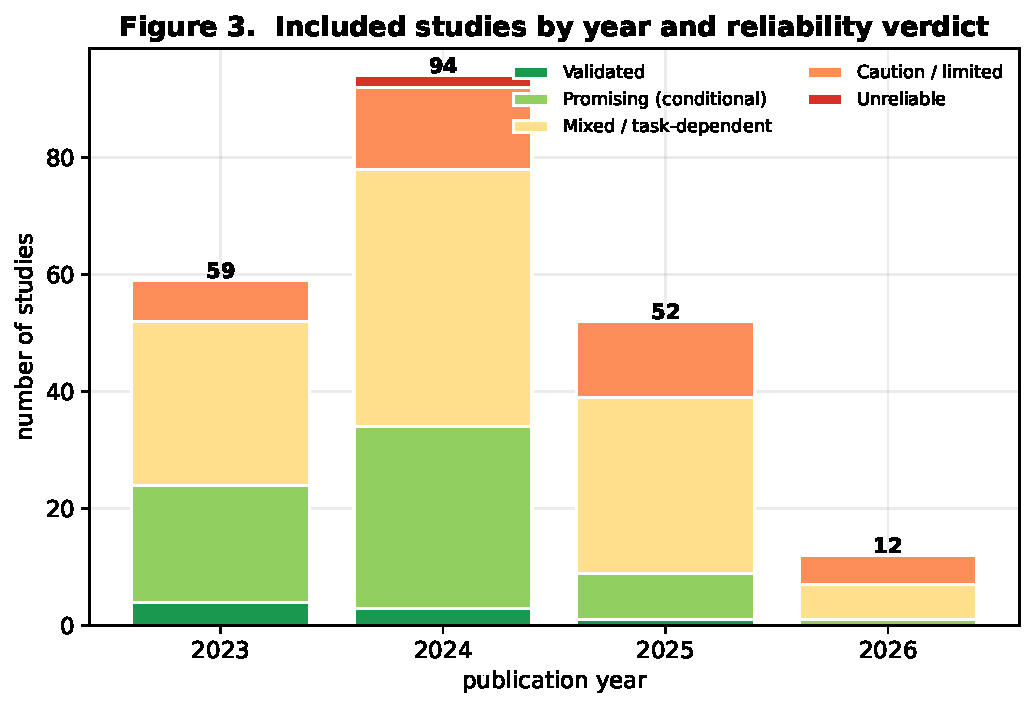
\includegraphics[width=\linewidth]{fig03_studies_per_year}\caption{}\label{fig:year}\end{subfigure}
\caption{Coverage: (a) studies per domain; (b) studies per year by verdict.}
\end{figure}
\begin{figure}[t]\centering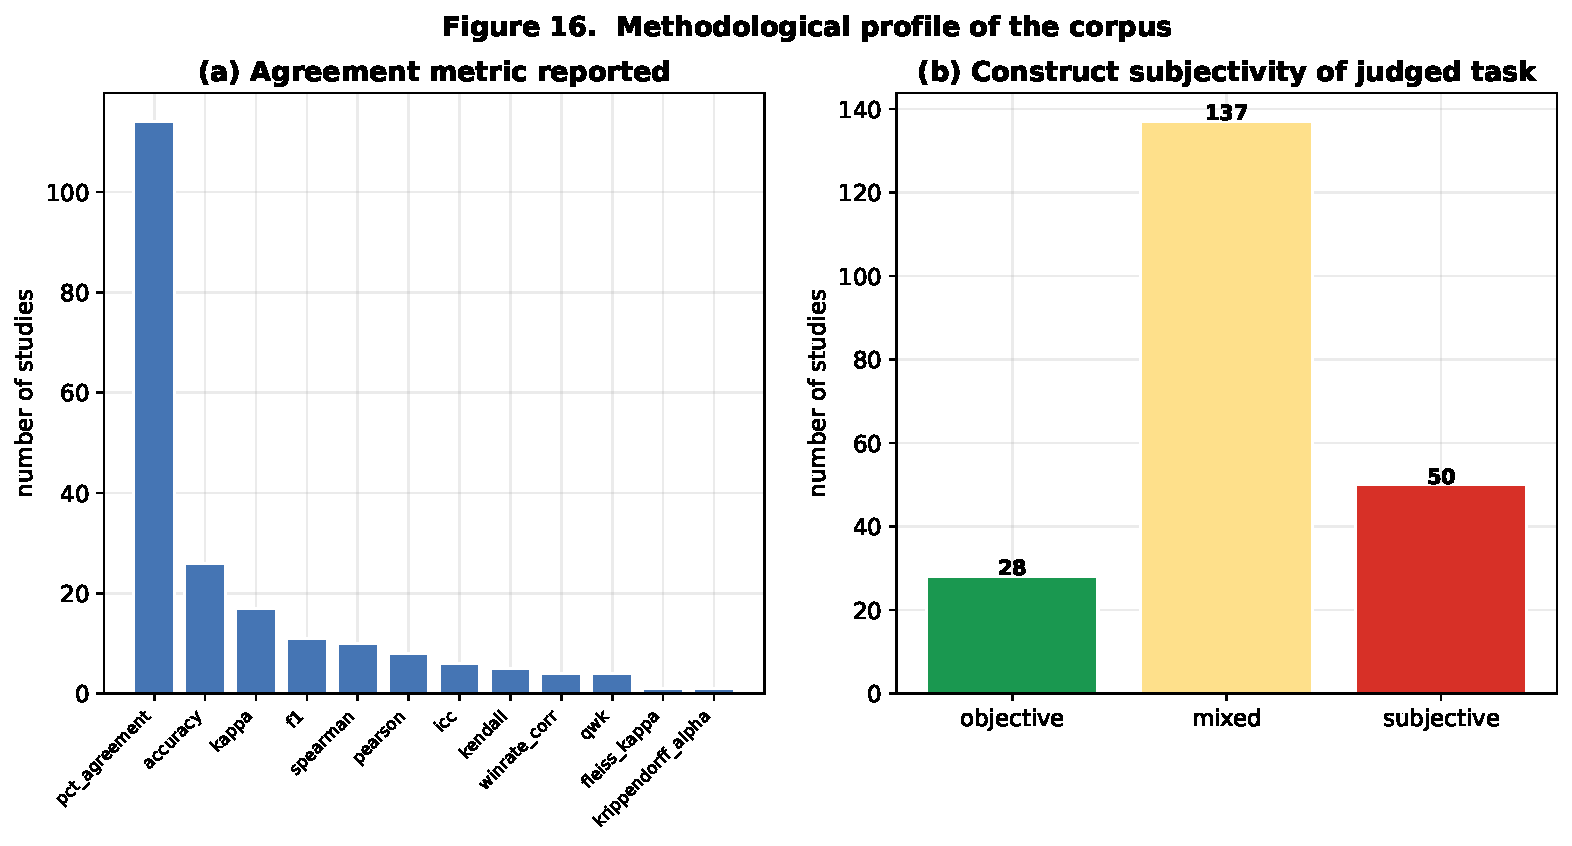
\includegraphics[width=\linewidth]{fig16_methodology}
\caption{Methodological profile: metric reported and construct subjectivity.}\label{fig:method}\end{figure}

\subsection{Overall and by domain}
The modal verdict is mixed; \Pctreliable\% reliable, \Pctproblematic\% problematic (mean \Meanrel/5;
Figure~\ref{fig:verdict}). \textbf{Green ($\ge$3.5; \Ngreen{} domains):} MT (system level), text-to-image,
instruction-following, QA/factuality, information extraction, general-NLG pairwise, dialogue, legal.
\textbf{Amber (\Namber):} summarization, RAG, education, social-science annotation, medicine (structure-dependent),
code, IR/relevance (contested \citep{clarke2024cantreplace,frobe2025assessorsagree}). \textbf{Red (\Nred):}
low-resource multilingual, creative writing. Family aggregates appear in Figure~\ref{fig:family}; the domain and
landscape views in Figures~\ref{fig:dom}--\ref{fig:land}; the decision table in Table~\ref{tab:decision}.

\begin{figure}[t]\centering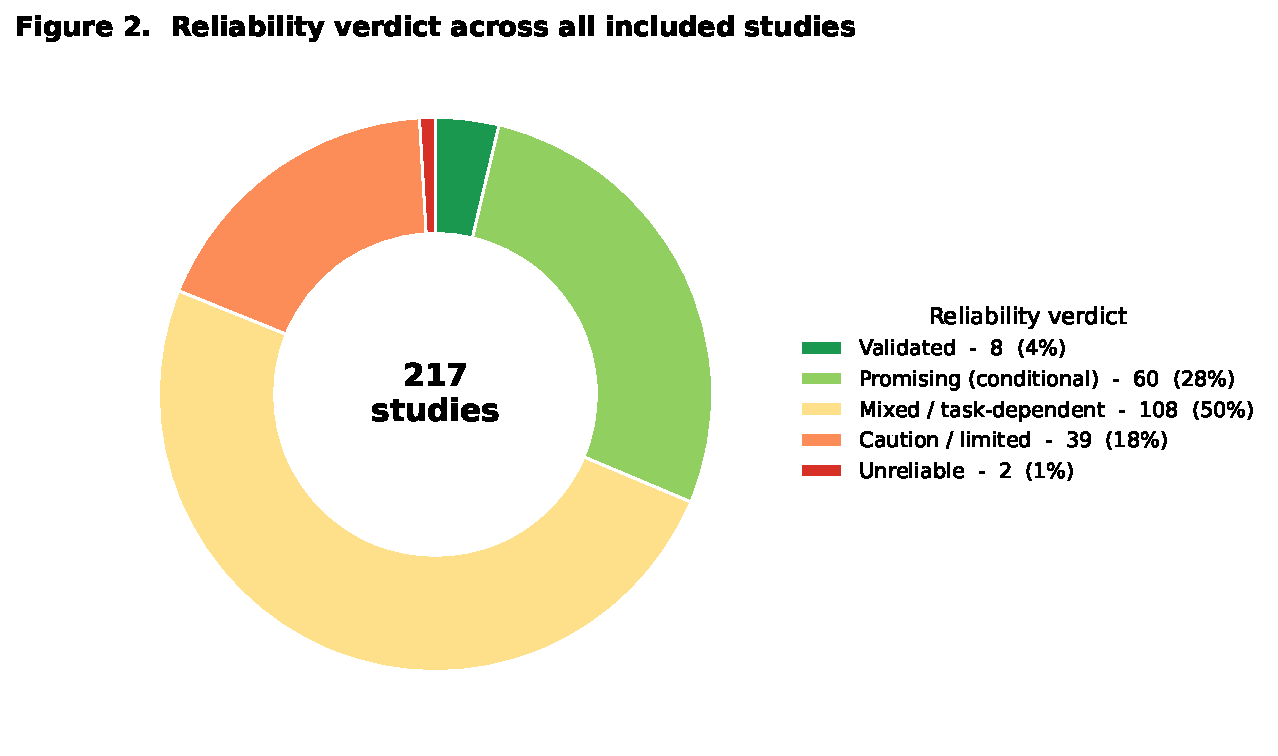
\includegraphics[width=0.8\linewidth]{fig02_verdict_overall}
\caption{Reliability verdict across all \Nstudies{} studies.}\label{fig:verdict}\end{figure}
\begin{figure}[t]\centering
\begin{subfigure}{0.5\linewidth}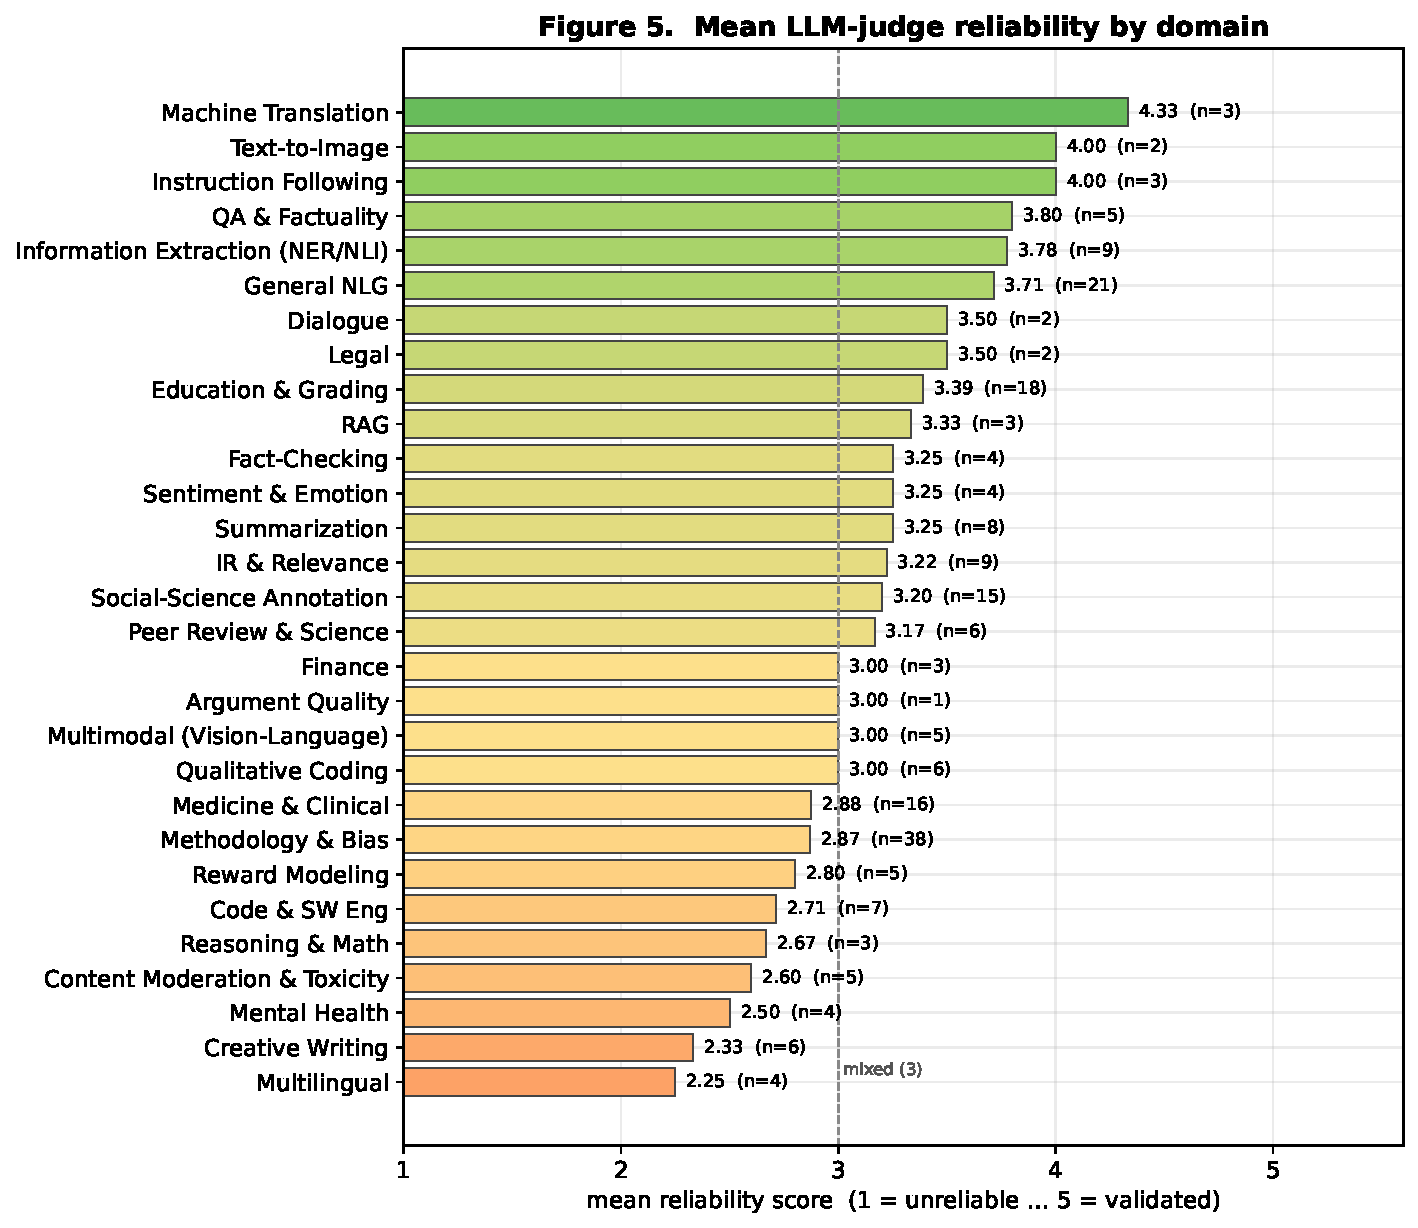
\includegraphics[width=\linewidth]{fig05_reliability_by_domain}\caption{}\label{fig:dom}\end{subfigure}\hfill
\begin{subfigure}{0.48\linewidth}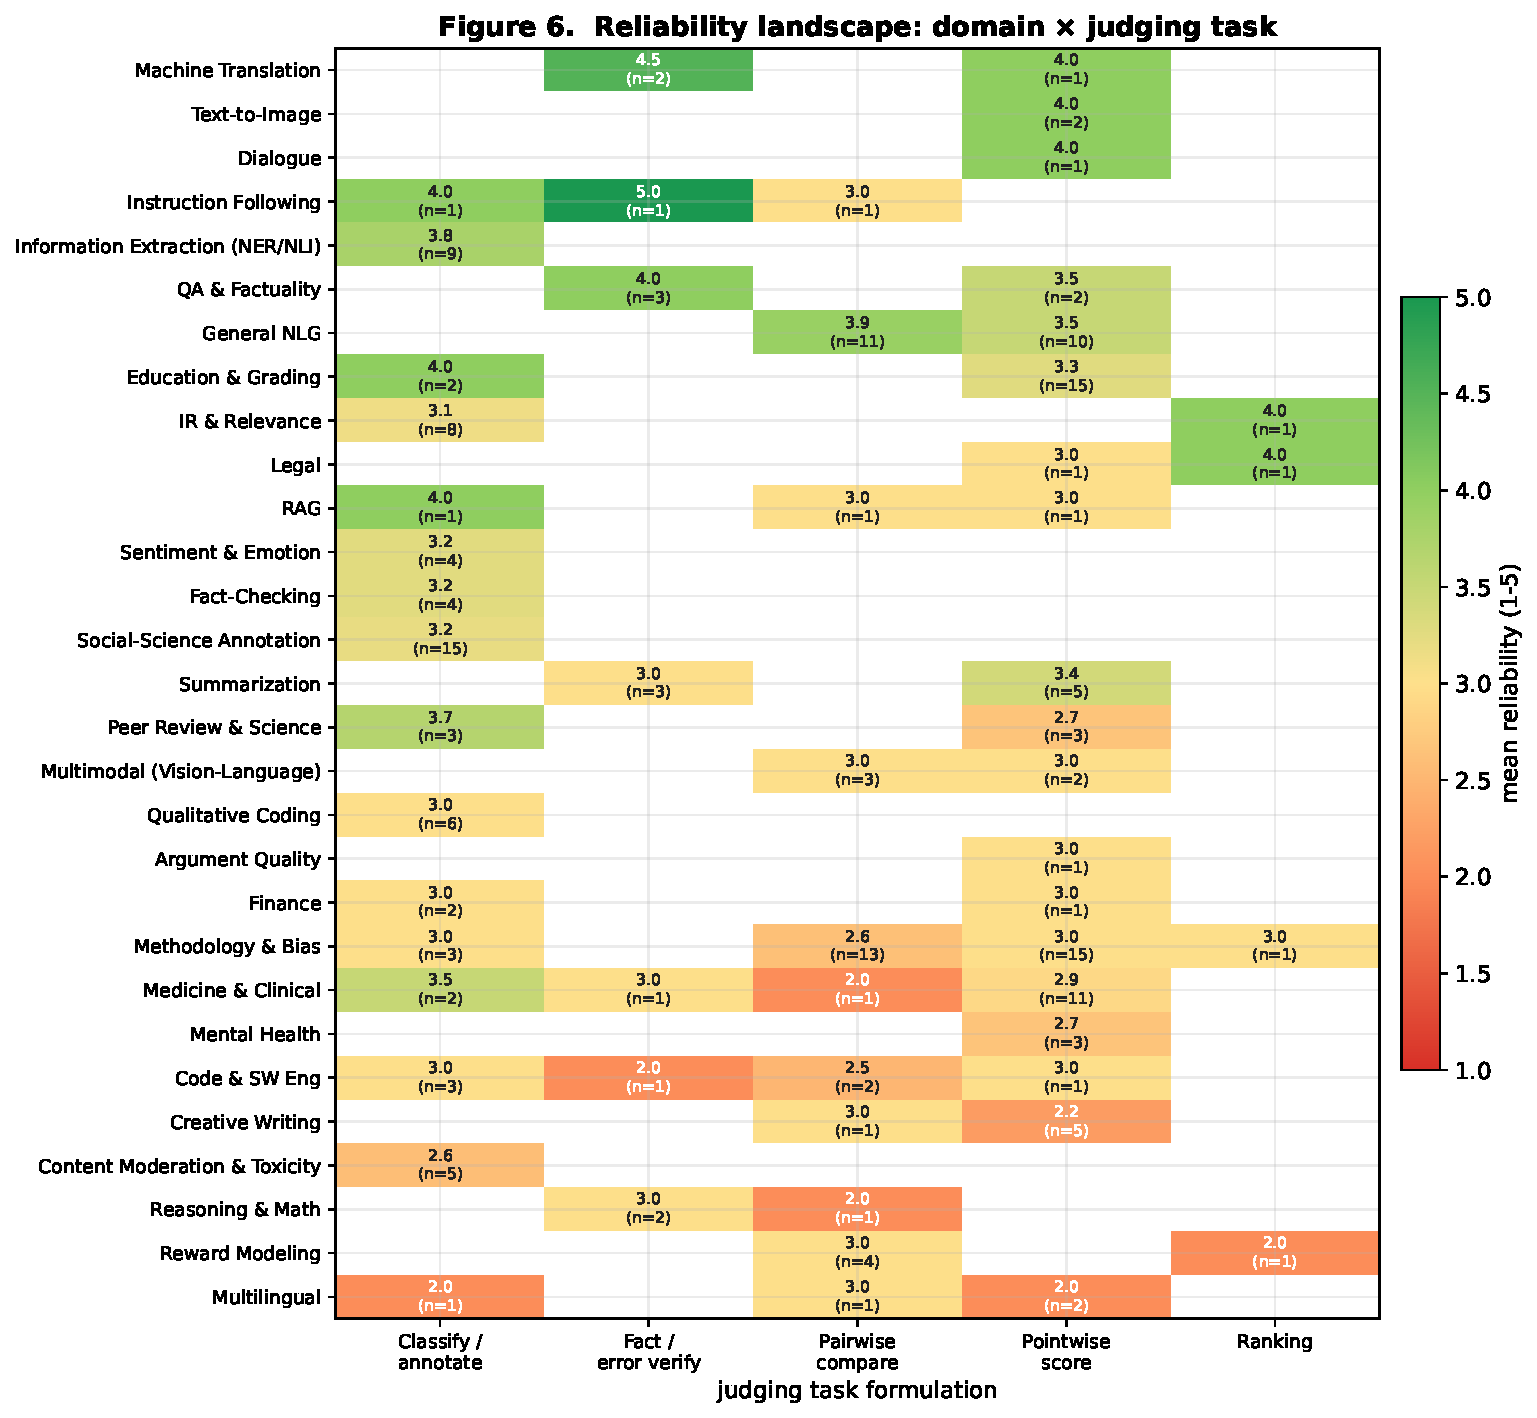
\includegraphics[width=\linewidth]{fig06_reliability_landscape}\caption{}\label{fig:land}\end{subfigure}
\caption{(a) Mean reliability by domain. (b) Domain$\times$task reliability landscape.}
\end{figure}
\begin{table}[tbp]\centering\small
\caption{Domain-level decision table. Mean reliability score (1 = unreliable $\dots$ 5 = validated), modal verdict,
and traffic-light signal (\textsc{green} $\ge 3.5$; \textsc{amber} 2.5-3.5; \textsc{red} $<2.5$). Sorted by mean
reliability. Small-$n$ domains should be read together with the family-level aggregates.}
\label{tab:decision}
\begin{tabular}{@{}l r c l c@{}}
\toprule
Domain / task & $n$ & Mean rel. & Modal verdict & Signal \\
\midrule
Machine Translation & 3 & 4.33 & Promising & \cellcolor{g!55}\textsc{green} \\
Text-to-Image & 2 & 4.00 & Promising & \cellcolor{g!55}\textsc{green} \\
Dialogue & 1 & 4.00 & Promising & \cellcolor{g!55}\textsc{green} \\
Instruction Following & 3 & 4.00 & Validated & \cellcolor{g!55}\textsc{green} \\
QA \& Factuality & 5 & 3.80 & Promising & \cellcolor{g!55}\textsc{green} \\
Information Extraction (NER/NLI) & 9 & 3.78 & Promising & \cellcolor{g!55}\textsc{green} \\
General NLG & 21 & 3.71 & Promising & \cellcolor{g!55}\textsc{green} \\
Legal & 2 & 3.50 & Promising & \cellcolor{g!55}\textsc{green} \\
Education \& Grading & 17 & 3.35 & Mixed & \cellcolor{a!60}\textsc{amber} \\
RAG & 3 & 3.33 & Mixed & \cellcolor{a!60}\textsc{amber} \\
Summarization & 8 & 3.25 & Promising & \cellcolor{a!60}\textsc{amber} \\
Fact-Checking & 4 & 3.25 & Promising & \cellcolor{a!60}\textsc{amber} \\
Sentiment \& Emotion & 4 & 3.25 & Mixed & \cellcolor{a!60}\textsc{amber} \\
IR \& Relevance & 9 & 3.22 & Promising & \cellcolor{a!60}\textsc{amber} \\
Social-Science Annotation & 15 & 3.20 & Mixed & \cellcolor{a!60}\textsc{amber} \\
Peer Review \& Science & 6 & 3.17 & Mixed & \cellcolor{a!60}\textsc{amber} \\
Multimodal (Vision-Language) & 5 & 3.00 & Mixed & \cellcolor{a!60}\textsc{amber} \\
Qualitative Coding & 6 & 3.00 & Mixed & \cellcolor{a!60}\textsc{amber} \\
Argument Quality & 1 & 3.00 & Mixed & \cellcolor{a!60}\textsc{amber} \\
Finance & 3 & 3.00 & Mixed & \cellcolor{a!60}\textsc{amber} \\
Medicine \& Clinical & 16 & 2.88 & Mixed & \cellcolor{a!60}\textsc{amber} \\
Methodology \& Bias & 38 & 2.87 & Mixed & \cellcolor{a!60}\textsc{amber} \\
Reward Modeling & 5 & 2.80 & Mixed & \cellcolor{a!60}\textsc{amber} \\
Code \& SW Eng & 7 & 2.71 & Mixed & \cellcolor{a!60}\textsc{amber} \\
Reasoning \& Math & 3 & 2.67 & Mixed & \cellcolor{a!60}\textsc{amber} \\
Content Moderation \& Toxicity & 5 & 2.60 & Mixed & \cellcolor{a!60}\textsc{amber} \\
Mental Health & 4 & 2.50 & Mixed & \cellcolor{a!60}\textsc{amber} \\
Creative Writing & 6 & 2.33 & Mixed & \cellcolor{r!55}\textsc{red} \\
Multilingual & 4 & 2.25 & Caution & \cellcolor{r!55}\textsc{red} \\
\bottomrule
\end{tabular}
\end{table}
\begin{figure}[t]\centering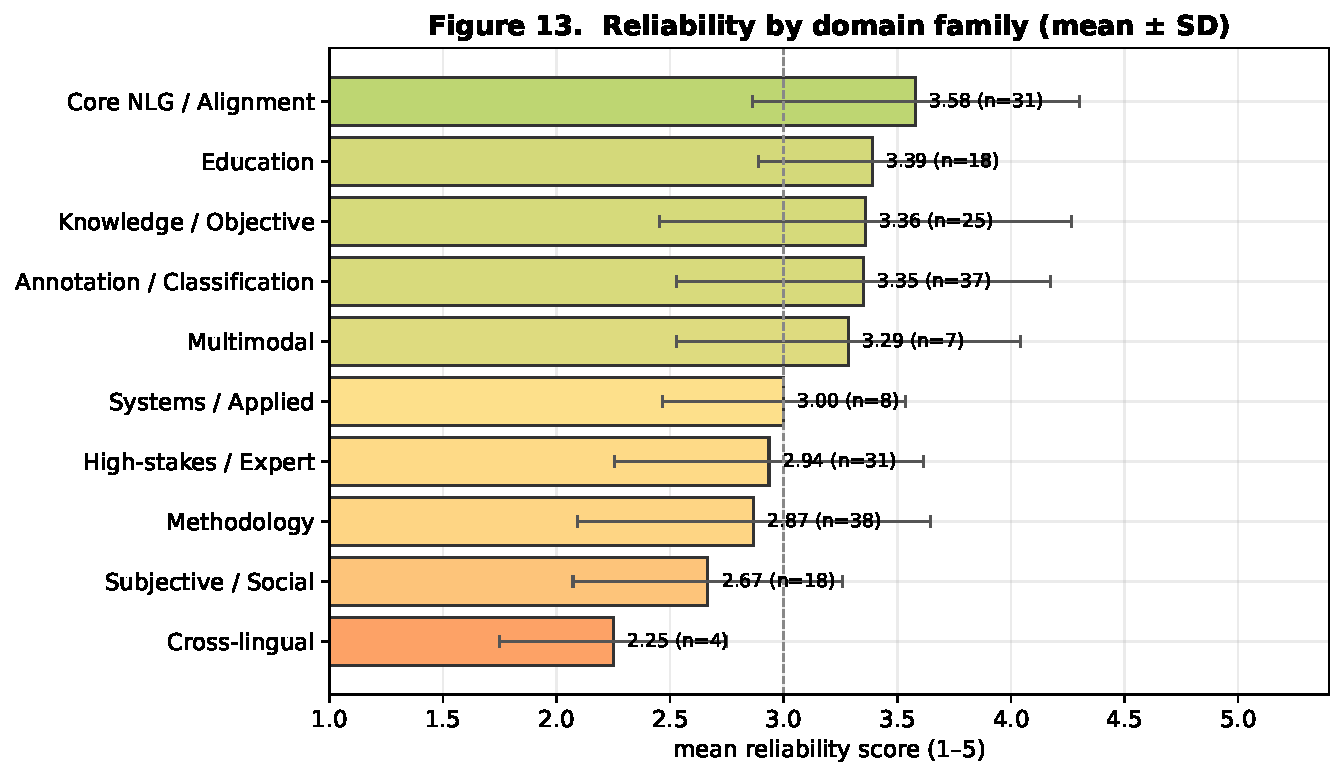
\includegraphics[width=0.82\linewidth]{fig13_family_reliability}
\caption{Reliability by domain family (mean$\pm$SD).}\label{fig:family}\end{figure}

\subsection{Task type, subjectivity, expertise}
Verification/classification tasks are more reliable than open-ended scoring (Figure~\ref{fig:subjexp}c); construct
subjectivity and required expertise both predict reliability monotonically (Figure~\ref{fig:subjexp}a,b), and judges
align better with non-experts than experts \citep{bavaresco2024judgebench,szymanski2025limits}.

\begin{figure}[t]\centering
\begin{subfigure}{0.32\linewidth}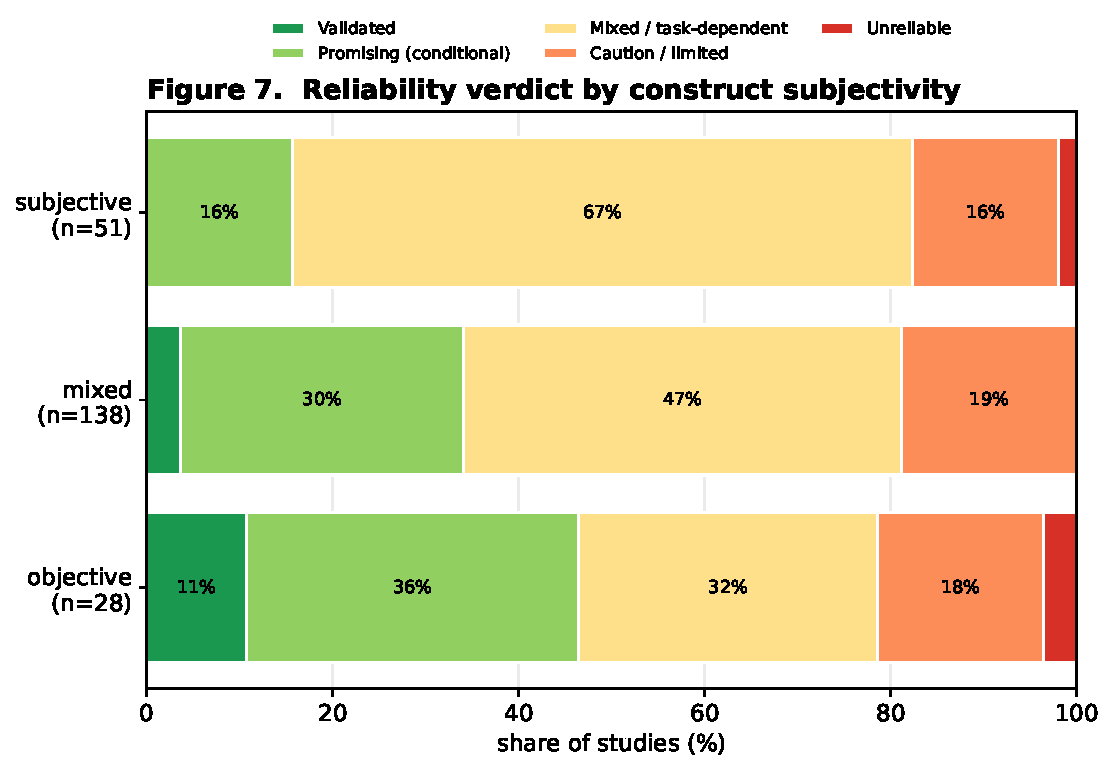
\includegraphics[width=\linewidth]{fig07_subjectivity}\caption{}\end{subfigure}\hfill
\begin{subfigure}{0.32\linewidth}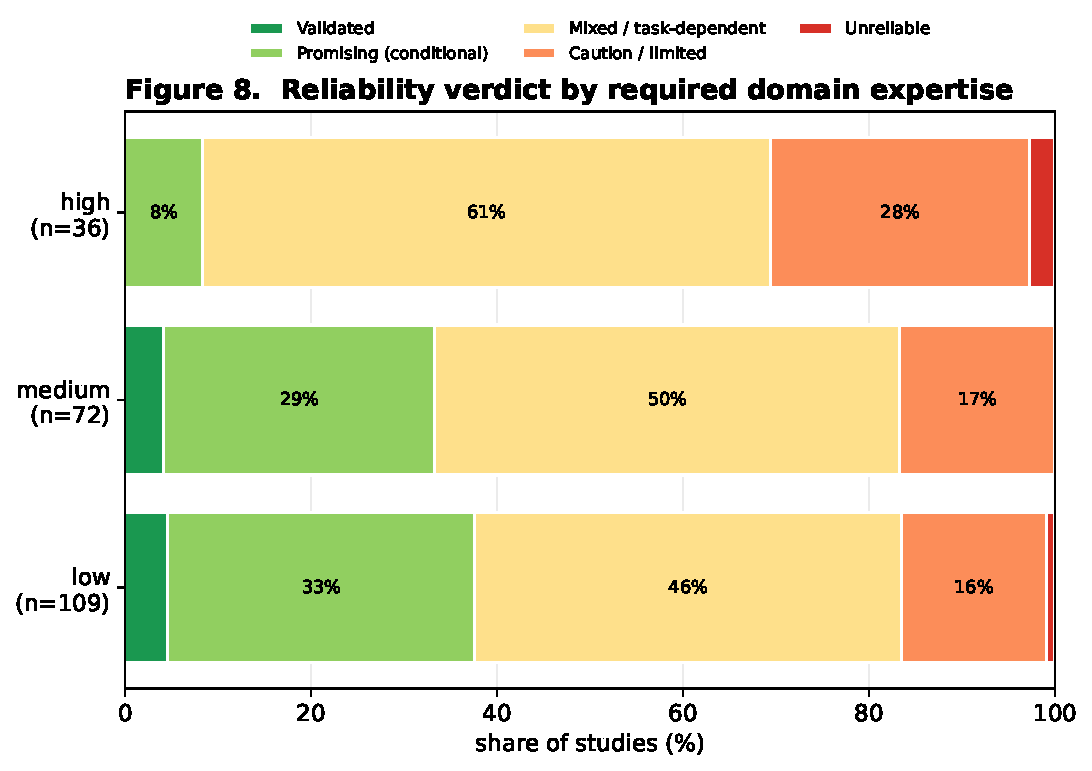
\includegraphics[width=\linewidth]{fig08_expertise}\caption{}\end{subfigure}\hfill
\begin{subfigure}{0.32\linewidth}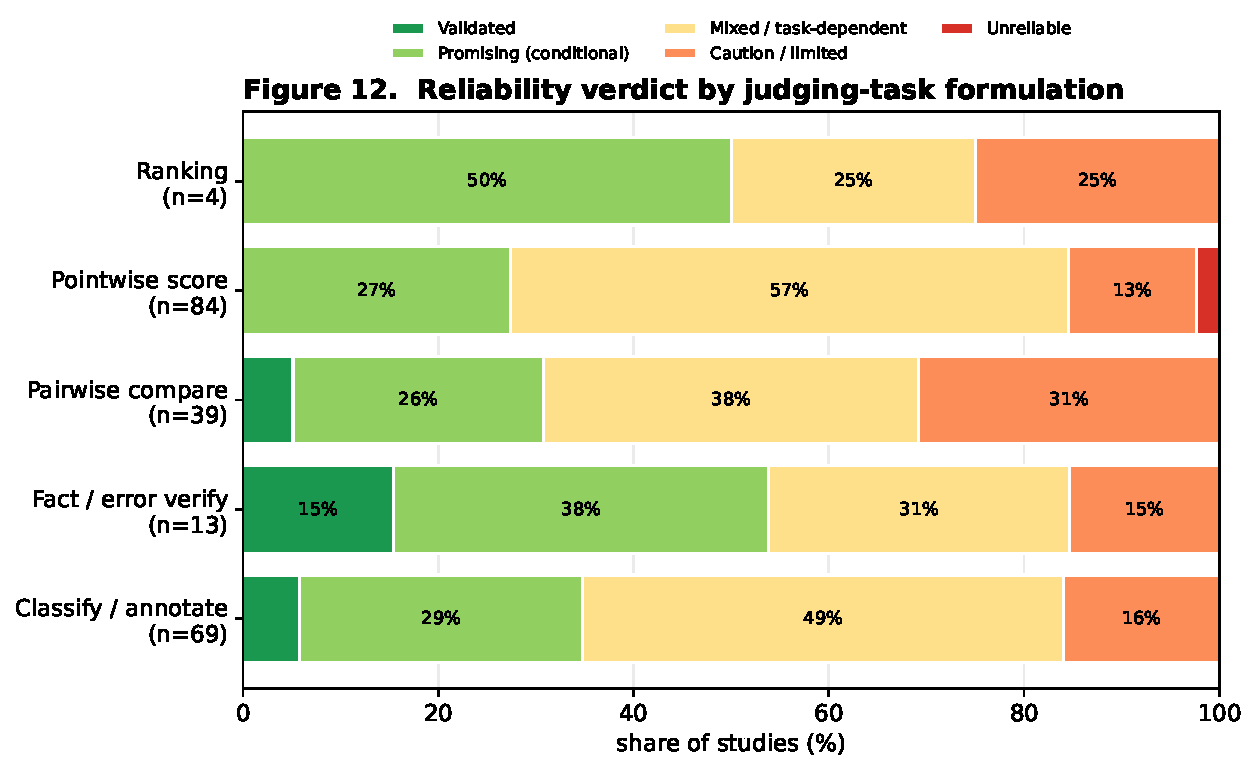
\includegraphics[width=\linewidth]{fig12_verdict_by_task}\caption{}\end{subfigure}
\caption{Verdict by (a) subjectivity, (b) expertise, (c) task formulation.}\label{fig:subjexp}
\end{figure}

\subsection{Agreement vs.\ the human ceiling}
The \Nnumeric{} studies with numeric values (Figure~\ref{fig:forest}) show the strongest results meet or exceed the
human ceiling---MT-Bench 85\% vs.\ 81\% \citep{zheng2023mtbench}, GEMBA-MQM 96.5\% \citep{kocmi2023gembamqm}, SAFE
wins 76\% of disagreements \citep{wei2024safe}, Prometheus Pearson 0.897 \citep{kim2023prometheus}, PRISMA screening
$\kappa>0.9$ \citep{prismascreen2024}---while the weakest fall far below (JUDGE-BENCH $\kappa=0.28$
\citep{bavaresco2024judgebench}). On subjective tasks the human ceiling is itself low ($\alpha<0.35$
\citep{imrit2026iaa}; Figure~\ref{fig:parity}; Table~\ref{tab:anchors}).

\begin{figure}[t]\centering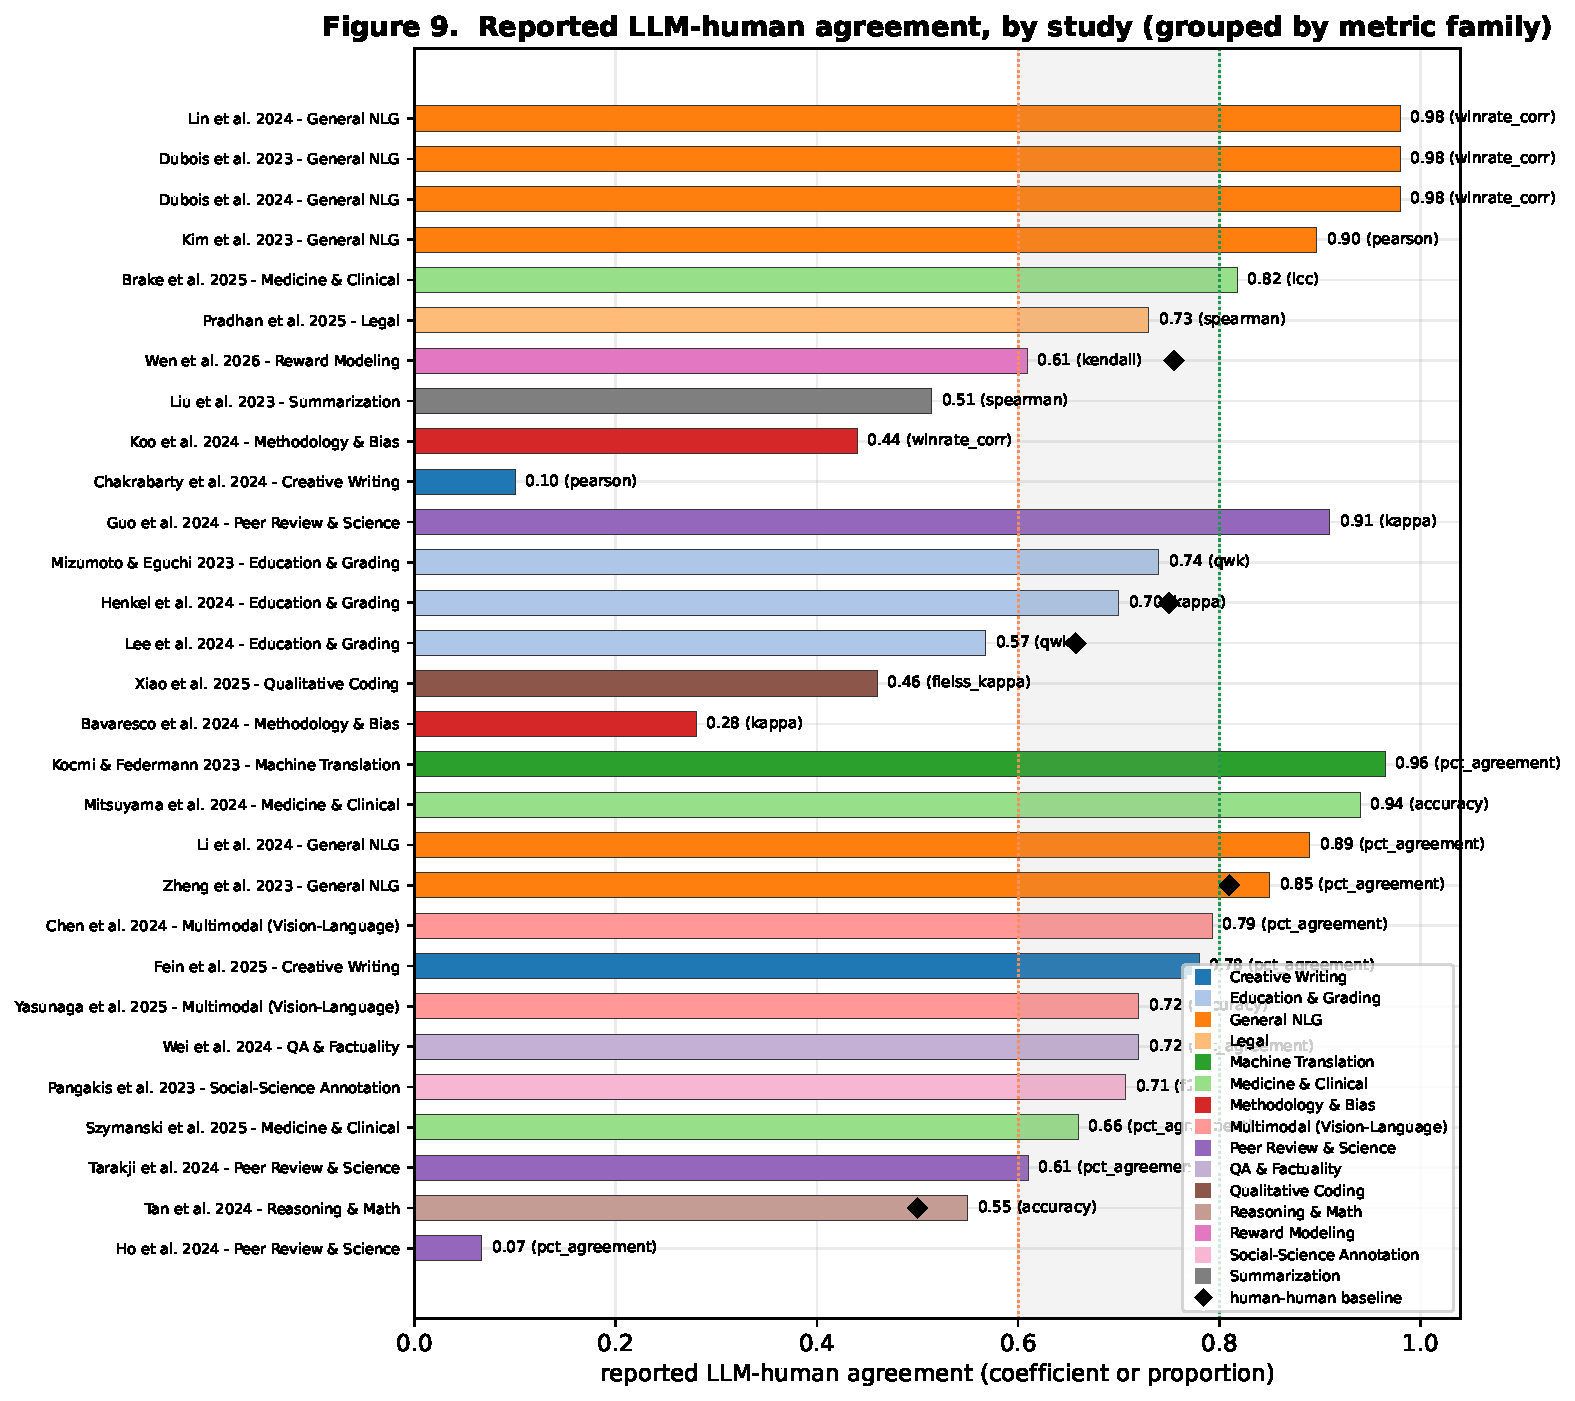
\includegraphics[width=0.9\linewidth]{fig09_agreement_forest}
\caption{Reported LLM--human agreement by study, grouped by metric family.}\label{fig:forest}\end{figure}
\begin{figure}[t]\centering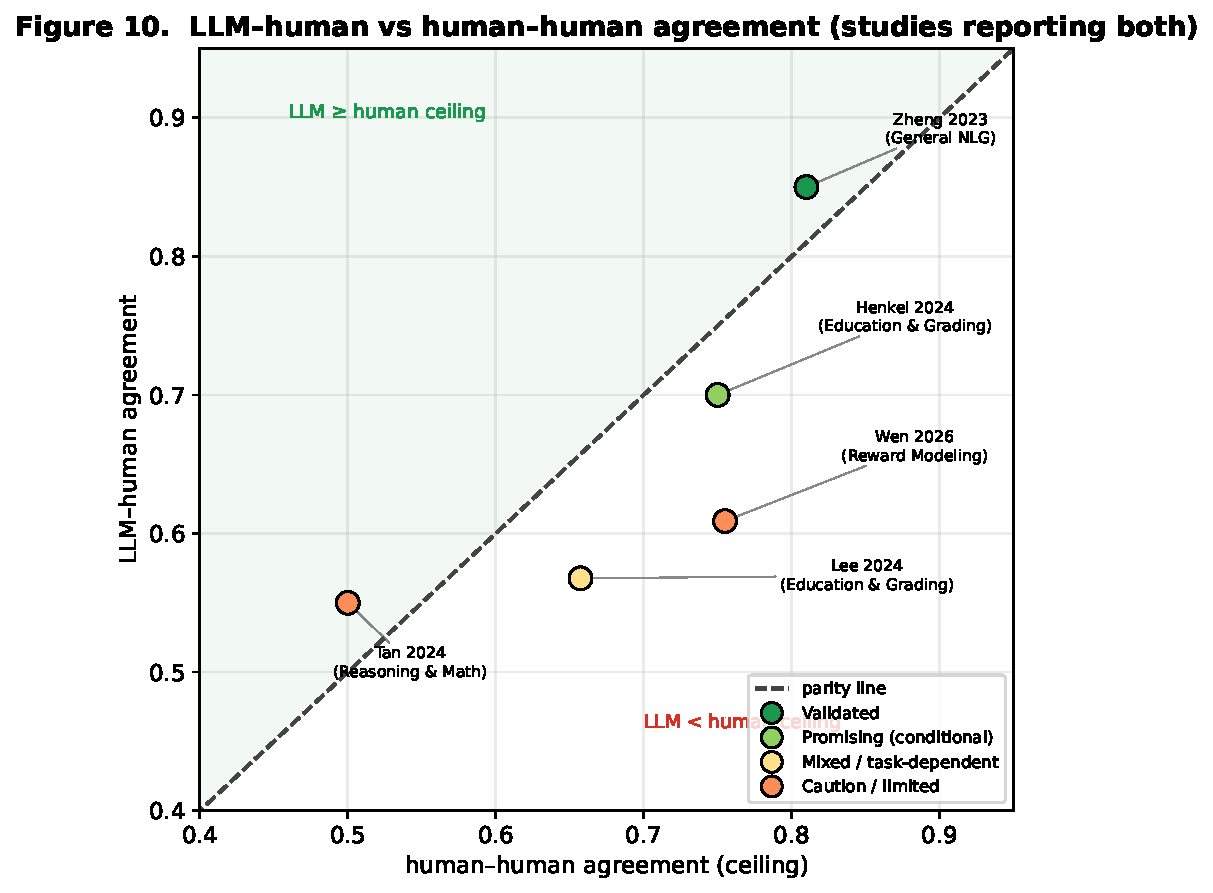
\includegraphics[width=0.72\linewidth]{fig10_parity_scatter}
\caption{LLM--human vs.\ human--human agreement.}\label{fig:parity}\end{figure}
\begin{table}[tbp]\centering\footnotesize
\caption{Quantitative anchors: studies reporting an extractable numeric LLM--human agreement value, with the
human--human baseline where reported. Metrics are heterogeneous (see \S\ref{sec:rubric}) and are interpreted
within metric families.}
\label{tab:anchors}
\begin{tabular}{@{}l l l c c l@{}}
\toprule
Study & Domain & Metric & LLM-human & Human-human & Verdict \\
\midrule
Chakrabarty et al. (2024) & Creative Writing & pearson & 0.10 &  & Unreliable \\
Fein et al. (2025) & Creative Writing & pct\_agreement & 0.78 &  & Mixed \\
Lee et al. (2024) & Education \& Grading & qwk & 0.57 & 0.66 & Mixed \\
Henkel et al. (2024) & Education \& Grading & kappa & 0.70 & 0.75 & Promising \\
Mizumoto \& Eguchi (2023) & Education \& Grading & qwk & 0.74 &  & Promising \\
Zheng et al. (2023) & General NLG & pct\_agreement & 0.85 & 0.81 & Validated \\
Li et al. (2024) & General NLG & pct\_agreement & 0.89 &  & Promising \\
Kim et al. (2023) & General NLG & pearson & 0.90 &  & Promising \\
Dubois et al. (2024) & General NLG & winrate\_corr & 0.98 &  & Promising \\
Dubois et al. (2023) & General NLG & winrate\_corr & 0.98 &  & Promising \\
Lin et al. (2024) & General NLG & winrate\_corr & 0.98 &  & Promising \\
Pradhan et al. (2025) & Legal & spearman & 0.73 &  & Promising \\
Kocmi \& Federmann (2023) & Machine Translation & pct\_agreement & 0.96 &  & Validated \\
Szymanski et al. (2025) & Medicine \& Clinical & pct\_agreement & 0.66 &  & Caution \\
Brake et al. (2025) & Medicine \& Clinical & icc & 0.82 &  & Mixed \\
Mitsuyama et al. (2024) & Medicine \& Clinical & accuracy & 0.94 &  & Mixed \\
Bavaresco et al. (2024) & Methodology \& Bias & kappa & 0.28 &  & Mixed \\
Koo et al. (2024) & Methodology \& Bias & winrate\_corr & 0.44 &  & Caution \\
Yasunaga et al. (2025) & Multimodal (Vision-Language) & accuracy & 0.72 &  & Caution \\
Chen et al. (2024) & Multimodal (Vision-Language) & pct\_agreement & 0.79 &  & Mixed \\
Ho et al. (2024) & Peer Review \& Science & pct\_agreement & 0.07 &  & Caution \\
Tarakji et al. (2024) & Peer Review \& Science & pct\_agreement & 0.61 &  & Mixed \\
Guo et al. (2024) & Peer Review \& Science & kappa & 0.91 &  & Validated \\
Wei et al. (2024) & QA \& Factuality & pct\_agreement & 0.72 &  & Promising \\
Xiao et al. (2025) & Qualitative Coding & fleiss\_kappa & 0.46 &  & Mixed \\
Tan et al. (2024) & Reasoning \& Math & accuracy & 0.55 & 0.50 & Caution \\
Wen et al. (2026) & Reward Modeling & kendall & 0.61 & 0.76 & Caution \\
Pangakis et al. (2023) & Social-Science Annotation & f1 & 0.71 &  & Mixed \\
Liu et al. (2023) & Summarization & spearman & 0.51 &  & Promising \\
\bottomrule
\end{tabular}
\end{table}

\subsection{Failure modes and moderators}
Recurring biases---verbosity/length \citep{dubois2024lc}, position \citep{zheng2023mtbench}, self-preference
\citep{panickssery2024selfpref,wataoka2024selfpref}, style-over-substance \citep{feuer2024style}, preference leakage
\citep{li2025prefleakage}, non-determinism \citep{temperature2026}, the expertise gap, and adversarial
manipulability \citep{raina2024robust}---modulate reliability (Figure~\ref{fig:bias}). Moderators: fine-tuned judges
excel in-domain but do not generalize \citep{zhu2023judgelm,huang2025empiricaljudge}; juries reduce bias
\citep{verga2024poll}; aggregate $\ne$ item-level reliability \citep{kocmi2023gembamqm}; low-resource languages
degrade sharply \citep{multiljudge2025}.

\begin{figure}[t]\centering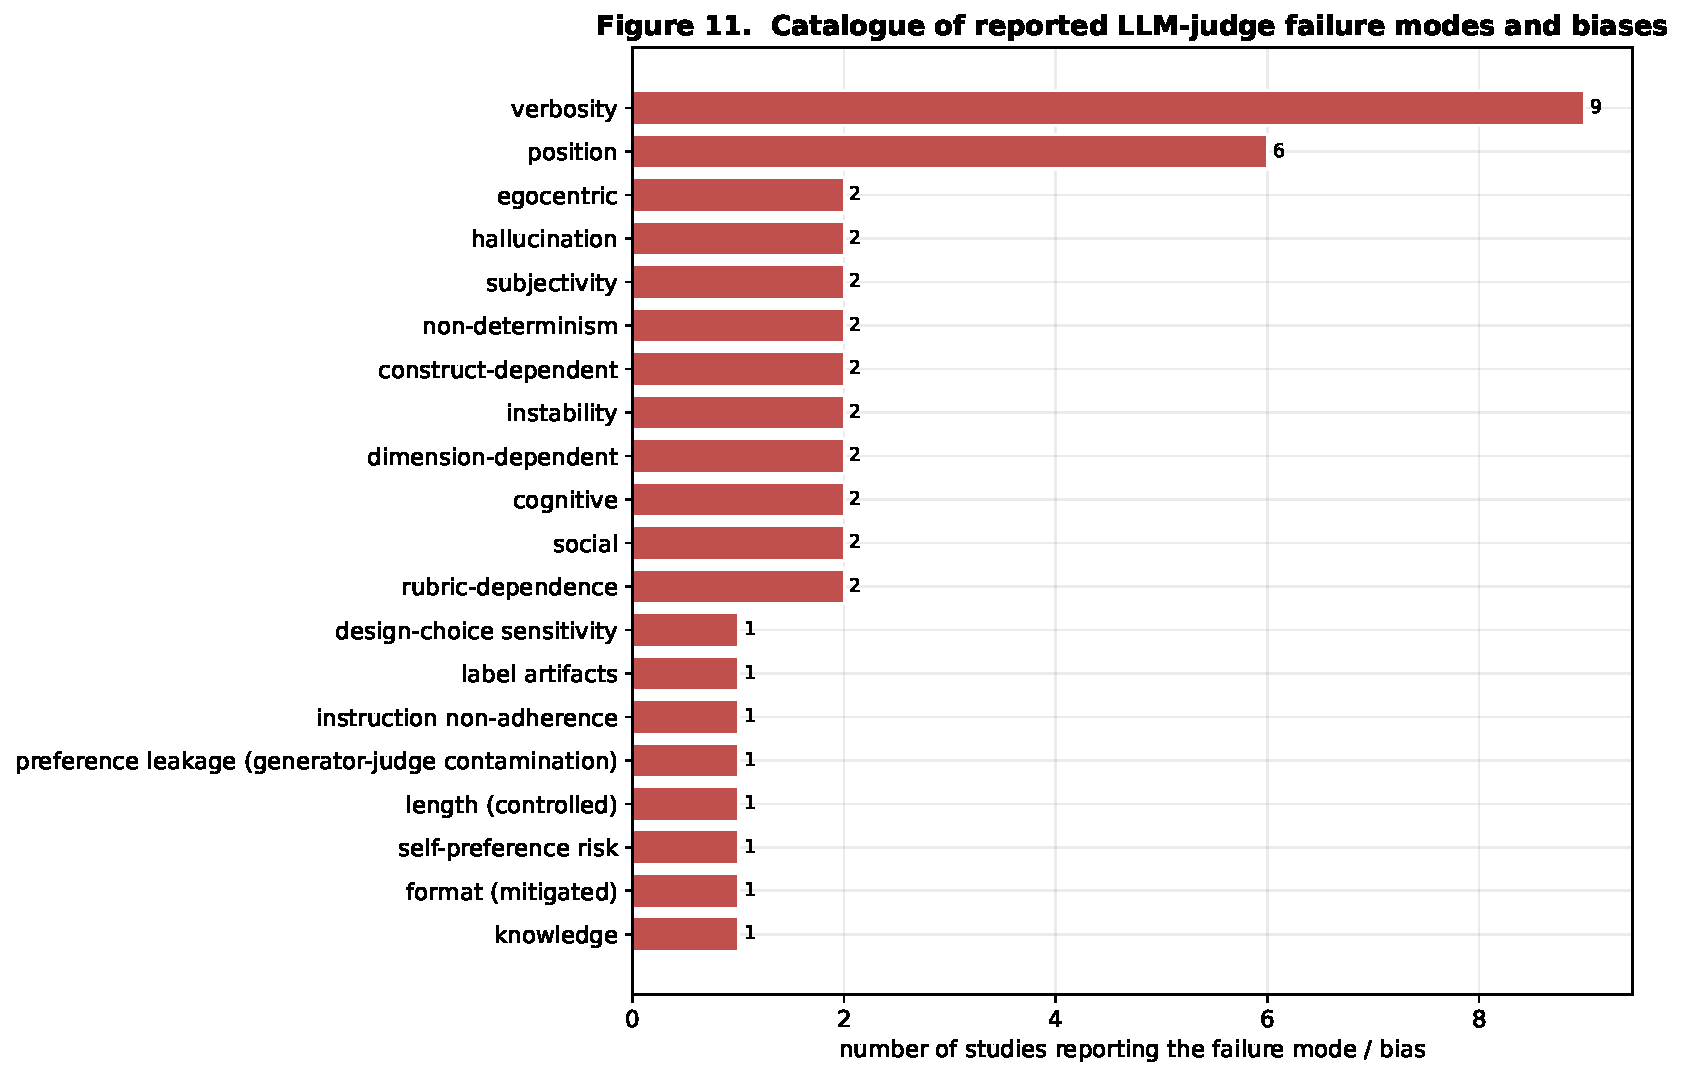
\includegraphics[width=0.9\linewidth]{fig11_bias_frequency}
\caption{Reported failure modes / biases (study counts).}\label{fig:bias}\end{figure}

\section{Discussion}
\textbf{Green zone (automate w/ light audit):} objective, verifiable, low-expertise tasks judged in aggregate.
\textbf{Amber zone (human-in-the-loop + per-task validation):} summarization, RAG, grading, social-science
annotation, peer review, structured clinical evaluation. \textbf{Red zone (keep humans):} subjective/expert/
low-resource/adversarial judgments. \emph{Architecture matters:} comparative $>$ absolute, juries $>$ single,
calibrated $>$ raw, fine-tuned $=$ in-domain specialist. The decision map (Figure~\ref{fig:decision}) and checklist
(Table~\ref{tab:checklist}) operationalize this.

\begin{figure}[t]\centering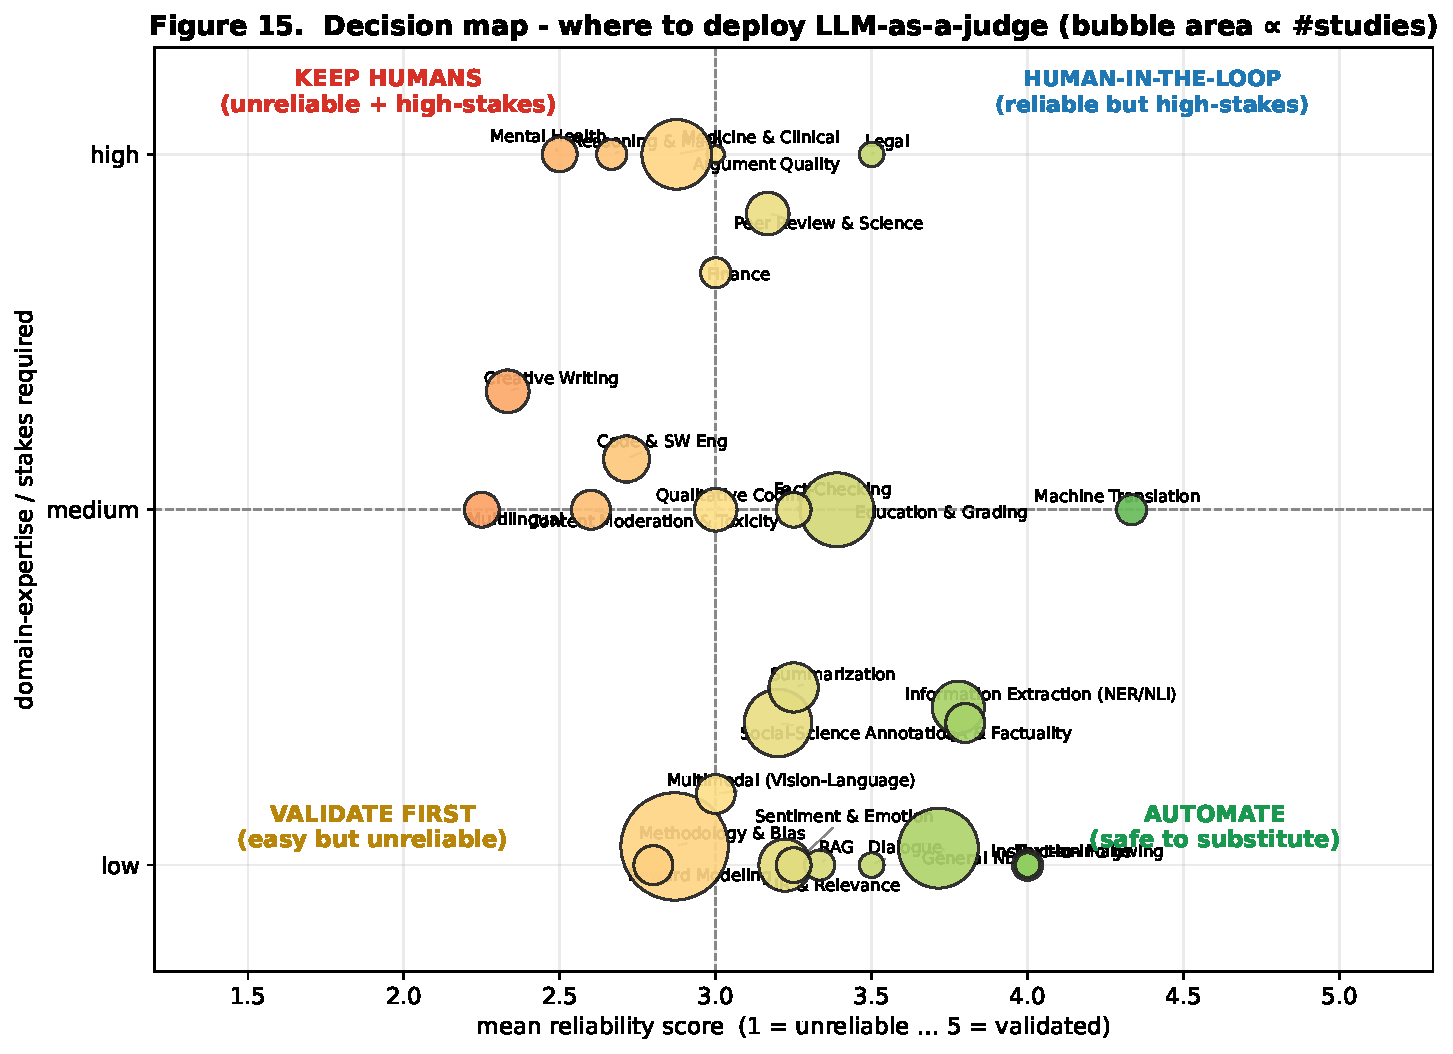
\includegraphics[width=\linewidth]{fig15_decision_map}
\caption{Deployment decision map (reliability$\times$stakes; bubble area $\propto$ studies).}\label{fig:decision}\end{figure}

\begin{table}[t]\centering\small
\caption{Validation checklist for trusting an LLM judge on a new task.}\label{tab:checklist}
\begin{tabular}{@{}p{0.62\linewidth} p{0.32\linewidth}@{}}
\toprule Question & If ``no''/unfavourable \\ \midrule
Objective with verifiable ground truth? & Expect verdict 3--5 \\
Low required expertise; non-expert labels suffice? & Beware expert--LLM gap \\
Human--human baseline known (``match a second human'')? & Run the alt-test \citep{calderon2025alttest} \\
Right granularity (item vs.\ system)? & Re-test at item level \\
Comparative (pairwise/jury) not absolute? & Prefer comparative \citep{verga2024poll} \\
Presentation biases controlled? & Debias \citep{dubois2024lc} \\
Generator and judge unrelated? & Avoid preference leakage \citep{li2025prefleakage} \\
Temperature/seed/version pinned? & Pin \citep{temperature2026} \\ \bottomrule
\end{tabular}\end{table}

\section{Limitations}
Single-reviewer LLM-assisted screening/extraction; heterogeneous metrics synthesized within families; small $n$ in
several domains; database recall depends on indexing; findings reflect mid-2026 models.

\section{Conclusion}
LLM-as-a-judge is a \emph{validated} substitute for objective, aggregate-level tasks, a \emph{conditional}
human-in-the-loop assistant for many applied domains, and an \emph{unsafe} replacement for subjective/expert/
low-resource/adversarial judgments. The right question is ``can this judge replace a second human on this task, at
this granularity, under these controls?''---answerable domain by domain.

\bibliographystyle{plainnat}
\bibliography{references}
\appendix
\section{Full extracted-studies corpus}\label{app:full}
{\footnotesize\footnotesize
\begin{longtable}{@{}l l l l l c l@{}}
\caption{Full extracted-studies corpus (217 included studies). Agreement is the headline coefficient/proportion where reported.}\label{tab:full}\\
\toprule
Key & Study & Domain & Task & Metric & Agree & Verdict \\
\midrule
\endfirsthead
\toprule Key & Study & Domain & Task & Metric & Agree & Verdict \\ \midrule \endhead
\texttt{mirzakhmedova2024argument} & Mirzakhmedova et al. (2024) & Argument Quality & pointwise & pct\_agreement & - & Mixed \\
\texttt{tong2024codejudge} & Tong et al. (2024) & Code \& SW Eng & classify & accuracy & - & Promising \\
\texttt{watson2024aicodereview} & Watson et al. (2024) & Code \& SW Eng & classify & pct\_agreement & - & Mixed \\
\texttt{codespec2025} & Jin et al. (2025) & Code \& SW Eng & verify & accuracy & - & Caution \\
\texttt{wang2025setesting} & Wang et al. (2025) & Code \& SW Eng & pairwise & pct\_agreement & - & Mixed \\
\texttt{zhuo2025codejudgeeff} & Wang et al. (2025) & Code \& SW Eng & pointwise & kappa & - & Mixed \\
\texttt{biasloop2026} & Zhao et al. (2026) & Code \& SW Eng & pairwise & pct\_agreement & - & Caution \\
\texttt{overcorrect2026} & Jin et al. (2026) & Code \& SW Eng & classify & accuracy & - & Caution \\
\texttt{hatespeechprobe2023} & Roy et al. (2023) & Content Moderation \& Toxicity & classify & f1 & - & Mixed \\
\texttt{li2023hotchatgpt} & Li et al. (2023) & Content Moderation \& Toxicity & classify & pct\_agreement & - & Mixed \\
\texttt{nguyen2024crisismisinfo} & Nguyen \& Rudra (2024) & Content Moderation \& Toxicity & classify & f1 & - & Mixed \\
\texttt{hatespeechanno2025} & authors (2025) & Content Moderation \& Toxicity & classify & kappa & - & Caution \\
\texttt{icwsm2025hatebias} & Giorgi et al. (2025) & Content Moderation \& Toxicity & classify & kappa & - & Caution \\
\texttt{xie2023nextchapter} & Xie et al. (2023) & Creative Writing & pointwise & pct\_agreement & - & Mixed \\
\texttt{chakrabarty2024artartifice} & Chakrabarty et al. (2024) & Creative Writing & pointwise & pearson & 0.10 & Unreliable \\
\texttt{ismayilzada2024creative} & Ismayilzada et al. (2024) & Creative Writing & pointwise & pct\_agreement & - & Caution \\
\texttt{creativeevalmdpi2025} & Kim et al. (2025) & Creative Writing & pointwise & spearman & - & Mixed \\
\texttt{haase2025creativitypeaked} & Haase et al. (2025) & Creative Writing & pointwise & pct\_agreement & - & Caution \\
\texttt{litbench2025} & Fein et al. (2025) & Creative Writing & pairwise & pct\_agreement & 0.78 & Mixed \\
\texttt{lin2023llmeval} & Lin \& Chen (2023) & Dialogue & pointwise & spearman & - & Promising \\
\texttt{mendonca2024dialogue} & Mendonca et al. (2024) & Dialogue & pointwise & spearman & - & Mixed \\
\texttt{hackl2023reliablerater} & Hackl et al. (2023) & Education \& Grading & pointwise & icc & - & Promising \\
\texttt{khademi2023bardassessment} & Khademi (2023) & Education \& Grading & pointwise & pct\_agreement & - & Mixed \\
\texttt{kortemeyer2023physics} & Kortemeyer (2023) & Education \& Grading & pointwise & pct\_agreement & - & Mixed \\
\texttt{mizumoto2023aes} & Mizumoto \& Eguchi (2023) & Education \& Grading & pointwise & qwk & 0.74 & Promising \\
\texttt{yancey2023cefr} & Yancey et al. (2023) & Education \& Grading & pointwise & qwk & - & Mixed \\
\texttt{aescomparative2024} & Lee et al. (2024) & Education \& Grading & pointwise & qwk & 0.57 & Mixed \\
\texttt{floden2024gradingexams} & Flodén (2024) & Education \& Grading & pointwise & pct\_agreement & - & Mixed \\
\texttt{grevisse2024asagmed} & Grévisse (2024) & Education \& Grading & classify & pct\_agreement & - & Promising \\
\texttt{hou2024classroom} & Hou et al. (2024) & Education \& Grading & pointwise & icc & - & Mixed \\
\texttt{k12shortanswer2024} & Henkel et al. (2024) & Education \& Grading & classify & kappa & 0.70 & Promising \\
\texttt{koraishi2024langassess} & Koraishi (2024) & Education \& Grading & pointwise & pct\_agreement & - & Mixed \\
\texttt{quah2024dentalaes} & Quah et al. (2024) & Education \& Grading & pointwise & icc & - & Mixed \\
\texttt{wang2024beyondagreement} & Wang et al. (2024) & Education \& Grading & pointwise & qwk & - & Mixed \\
\texttt{writingmultidim2024} & Steiss et al. (2024) & Education \& Grading & pointwise & qwk & - & Promising \\
\texttt{asagfair2025} & Henkel et al. (2025) & Education \& Grading & pointwise & kappa & - & Mixed \\
\texttt{sefl2025feedback} & authors (2025) & Education \& Grading & pointwise & f1 & - & Promising \\
\texttt{studentsjudge2025} & Banihashem et al. (2025) & Education \& Grading & pointwise & pct\_agreement & - & Mixed \\
\texttt{k12sci2026} & He et al. (2026) & Education \& Grading & pointwise & pct\_agreement & - & Promising \\
\texttt{claimmatch2023} & Choi et al. (2023) & Fact-Checking & classify & pct\_agreement & - & Promising \\
\texttt{ni2024afacta} & Ni et al. (2024) & Fact-Checking & classify & pct\_agreement & - & Promising \\
\texttt{politicaltruths2024} & Chatrath et al. (2024) & Fact-Checking & classify & pct\_agreement & - & Mixed \\
\texttt{factsopinions2025} & Saju et al. (2025) & Fact-Checking & classify & accuracy & - & Caution \\
\texttt{kaikaus2023financecorpora} & Kaikaus et al. (2023) & Finance & classify & accuracy & - & Mixed \\
\texttt{bizfinbench2025} & Lu et al. (2025) & Finance & pointwise & pct\_agreement & - & Mixed \\
\texttt{trident2025} & Hui et al. (2025) & Finance & classify & pct\_agreement & - & Mixed \\
\texttt{chan2023chateval} & Chan et al. (2023) & General NLG & pairwise & pct\_agreement & - & Mixed \\
\texttt{chiang2023alt} & Chiang \& Lee (2023) & General NLG & pointwise & pct\_agreement & - & Mixed \\
\texttt{dubois2023alpacafarm} & Dubois et al. (2023) & General NLG & pairwise & winrate\_corr & 0.98 & Promising \\
\texttt{hsu2023figurecaption} & Hsu et al. (2023) & General NLG & pointwise & spearman & - & Promising \\
\texttt{kim2023prometheus} & Kim et al. (2023) & General NLG & pointwise & pearson & 0.90 & Promising \\
\texttt{lai2023styletransfer} & Lai et al. (2023) & General NLG & pointwise & spearman & - & Mixed \\
\texttt{li2023autoj} & Li et al. (2023) & General NLG & pairwise & pct\_agreement & - & Mixed \\
\texttt{wang2023chatgptnlg} & Wang et al. (2023) & General NLG & pointwise & spearman & - & Mixed \\
\texttt{wang2023pandalm} & Wang et al. (2023) & General NLG & pairwise & accuracy & - & Promising \\
\texttt{xu2023instructscore} & Xu et al. (2023) & General NLG & pointwise & pearson & - & Promising \\
\texttt{zhang2023widerdeeper} & Zhang et al. (2023) & General NLG & pairwise & pct\_agreement & - & Mixed \\
\texttt{zheng2023mtbench} & Zheng et al. (2023) & General NLG & pairwise & pct\_agreement & 0.85 & Validated \\
\texttt{chiang2024arena} & Chiang et al. (2024) & General NLG & pairwise & pct\_agreement & - & Validated \\
\texttt{doostmohammadi2024autoeval} & Doostmohammadi et al. (2024) & General NLG & pointwise & pct\_agreement & - & Mixed \\
\texttt{dubois2024lc} & Dubois et al. (2024) & General NLG & pairwise & winrate\_corr & 0.98 & Promising \\
\texttt{hashemi2024llmrubric} & Hashemi et al. (2024) & General NLG & pointwise & pearson & - & Promising \\
\texttt{huang2024nlexpl} & Huang et al. (2024) & General NLG & pointwise & pct\_agreement & - & Mixed \\
\texttt{kim2024prometheus2} & Kim et al. (2024) & General NLG & pointwise & pearson & - & Promising \\
\texttt{li2024arenahard} & Li et al. (2024) & General NLG & pairwise & pct\_agreement & 0.89 & Promising \\
\texttt{lin2024wildbench} & Lin et al. (2024) & General NLG & pairwise & winrate\_corr & 0.98 & Promising \\
\texttt{verga2024poll} & Verga et al. (2024) & General NLG & pairwise & pct\_agreement & - & Promising \\
\texttt{faggioli2023perspectives} & Faggioli et al. (2023) & IR \& Relevance & classify & kappa & - & Promising \\
\texttt{alaofi2024fooledrelevant} & Alaofi et al. (2024) & IR \& Relevance & classify & pct\_agreement & - & Caution \\
\texttt{clarke2024cantreplace} & Clarke \& Dietz (2024) & IR \& Relevance & classify & kappa & - & Caution \\
\texttt{thomas2024relevance} & Thomas et al. (2024) & IR \& Relevance & classify & kappa & - & Validated \\
\texttt{upadhyay2024largescale} & Upadhyay et al. (2024) & IR \& Relevance & classify & kappa & - & Promising \\
\texttt{zhuang2024beyondyesno} & Zhuang et al. (2024) & IR \& Relevance & ranking & kendall & - & Promising \\
\texttt{arabzadeh2025benchrelevance} & Arabzadeh \& Clarke (2025) & IR \& Relevance & classify & kappa & - & Mixed \\
\texttt{arabzadeh2025promptsens} & Arabzadeh \& Clarke (2025) & IR \& Relevance & classify & kappa & - & Mixed \\
\texttt{frobe2025assessorsagree} & Frobe et al. (2025) & IR \& Relevance & classify & kappa & - & Caution \\
\texttt{li2023coannotating} & Li et al. (2023) & Information Extraction (NER/NLI) & classify & pct\_agreement & - & Promising \\
\texttt{humanllmcollab2024} & Wang et al. (2024) & Information Extraction (NER/NLI) & classify & pct\_agreement & - & Promising \\
\texttt{kholodna2024activelearning} & Kholodna et al. (2024) & Information Extraction (NER/NLI) & classify & f1 & - & Promising \\
\texttt{kim2024meganno} & Kim et al. (2024) & Information Extraction (NER/NLI) & classify & f1 & - & Promising \\
\texttt{nasution2024chatgptlabel} & Nasution \& Onan (2024) & Information Extraction (NER/NLI) & classify & accuracy & - & Mixed \\
\texttt{ner2024augment} & Naraki et al. (2024) & Information Extraction (NER/NLI) & classify & f1 & - & Promising \\
\texttt{nli2024labeldist} & Chen et al. (2024) & Information Extraction (NER/NLI) & classify & pearson & - & Promising \\
\texttt{ronningstad2024gptannotator} & Ronningstad et al. (2024) & Information Extraction (NER/NLI) & classify & f1 & - & Mixed \\
\texttt{qiu2025labelensemble} & Qiu et al. (2025) & Information Extraction (NER/NLI) & classify & accuracy & - & Promising \\
\texttt{zhou2023ifeval} & Zhou et al. (2023) & Instruction Following & verify & accuracy & - & Validated \\
\texttt{zeng2024llmbar} & Zeng et al. (2024) & Instruction Following & pairwise & accuracy & - & Mixed \\
\texttt{ifcritic2025} & Wen et al. (2025) & Instruction Following & classify & pct\_agreement & - & Promising \\
\texttt{legaldocrec2025} & Pradhan et al. (2025) & Legal & ranking & spearman & 0.73 & Promising \\
\texttt{lemaj2025} & Enguehard et al. (2025) & Legal & pointwise & pct\_agreement & - & Mixed \\
\texttt{kocmi2023gemba} & Kocmi \& Federmann (2023) & Machine Translation & pointwise & kendall & - & Promising \\
\texttt{kocmi2023gembamqm} & Kocmi \& Federmann (2023) & Machine Translation & verify & pct\_agreement & 0.96 & Validated \\
\texttt{lu2023erroranalysis} & Lu et al. (2023) & Machine Translation & verify & kendall & - & Promising \\
\texttt{sun2023radimpressions} & Sun et al. (2023) & Medicine \& Clinical & pointwise & pct\_agreement & - & Caution \\
\texttt{tang2023medevidence} & Tang et al. (2023) & Medicine \& Clinical & pointwise & pct\_agreement & - & Caution \\
\texttt{brain2024radgpt} & Mitsuyama et al. (2024) & Medicine \& Clinical & classify & accuracy & 0.94 & Mixed \\
\texttt{brake2024clinicalnote} & Brake \& Schaaf (2024) & Medicine \& Clinical & pointwise & pct\_agreement & - & Mixed \\
\texttt{wang2024clinicalevent} & Wang et al. (2024) & Medicine \& Clinical & classify & pct\_agreement & - & Promising \\
\texttt{chung2025verifact} & Chung et al. (2025) & Medicine \& Clinical & verify & pct\_agreement & - & Mixed \\
\texttt{clinstruct2025} & Brake et al. (2025) & Medicine \& Clinical & pointwise & icc & 0.82 & Mixed \\
\texttt{croxford2025autoeval} & Croxford et al. (2025) & Medicine \& Clinical & pointwise & pct\_agreement & - & Mixed \\
\texttt{croxford2025clinsummjudge} & Croxford et al. (2025) & Medicine \& Clinical & pointwise & pct\_agreement & - & Mixed \\
\texttt{healthbench2025} & Arora et al. (OpenAI) (2025) & Medicine \& Clinical & pointwise & pct\_agreement & - & Promising \\
\texttt{kim2025emulate} & Kim \& Kim (2025) & Medicine \& Clinical & pointwise & pct\_agreement & - & Mixed \\
\texttt{llmevalmed2025} & Zhang et al. (2025) & Medicine \& Clinical & pointwise & pct\_agreement & - & Mixed \\
\texttt{szymanski2025limits} & Szymanski et al. (2025) & Medicine \& Clinical & pairwise & pct\_agreement & 0.66 & Caution \\
\texttt{clindialog2026} & Sun et al. (2026) & Medicine \& Clinical & pointwise & pct\_agreement & - & Mixed \\
\texttt{frenchmedqa2026} & Belmadani et al. (2026) & Medicine \& Clinical & pointwise & kappa & - & Mixed \\
\texttt{medjudge2026scoping} & Li et al. (2026) & Medicine \& Clinical & review & nan & - & Caution \\
\texttt{counselbench2025} & Li et al. (2025) & Mental Health & pointwise & pct\_agreement & - & Caution \\
\texttt{hua2025mhscoping} & Hua et al. (2025) & Mental Health & review & nan & - & Caution \\
\texttt{mhtrust2025} & Badawi et al. (2025) & Mental Health & pointwise & icc & - & Mixed \\
\texttt{mhsupport2026} & Badawi et al. (2026) & Mental Health & pointwise & icc & - & Mixed \\
\texttt{liu2023trustworthy} & Liu et al. (2023) & Methodology \& Bias & survey & nan & - & Mixed \\
\texttt{saito2023verbositybias} & Saito et al. (2023) & Methodology \& Bias & pairwise & pct\_agreement & - & Caution \\
\texttt{wang2023shepherd} & Wang et al. (2023) & Methodology \& Bias & pointwise & pct\_agreement & - & Promising \\
\texttt{zhu2023judgelm} & Zhu et al. (2023) & Methodology \& Bias & pairwise & pct\_agreement & - & Promising \\
\texttt{bavaresco2024judgebench} & Bavaresco et al. (2024) & Methodology \& Bias & classify & kappa & 0.28 & Mixed \\
\texttt{chen2024humansorllms} & Chen et al. (2024) & Methodology \& Bias & pairwise & pct\_agreement & - & Caution \\
\texttt{desmond2024evalullm} & Desmond et al. (2024) & Methodology \& Bias & pointwise & pct\_agreement & - & Mixed \\
\texttt{fan2024sedareval} & Fan et al. (2024) & Methodology \& Bias & pointwise & pct\_agreement & - & Promising \\
\texttt{feuer2024style} & Feuer et al. (2024) & Methodology \& Bias & pairwise & pct\_agreement & - & Caution \\
\texttt{gu2024survey} & Gu et al. (2024) & Methodology \& Bias & survey & nan & - & Mixed \\
\texttt{jung2024trustescalate} & Jung et al. (2024) & Methodology \& Bias & pairwise & pct\_agreement & - & Promising \\
\texttt{justice2024prejudice} & Ye et al. (2024) & Methodology \& Bias & pairwise & pct\_agreement & - & Caution \\
\texttt{ke2024critiquellm} & Ke et al. (2024) & Methodology \& Bias & pointwise & spearman & - & Mixed \\
\texttt{koo2024cobbler} & Koo et al. (2024) & Methodology \& Bias & pairwise & winrate\_corr & 0.44 & Caution \\
\texttt{li2024compsurvey} & Li et al. (2024) & Methodology \& Bias & survey & nan & - & Mixed \\
\texttt{li2024gen2judge} & Li et al. (2024) & Methodology \& Bias & survey & nan & - & Mixed \\
\texttt{li2024splitmerge} & Li et al. (2024) & Methodology \& Bias & pairwise & pct\_agreement & - & Mixed \\
\texttt{liu2024pairwisepref} & Liu et al. (2024) & Methodology \& Bias & pairwise & pct\_agreement & - & Promising \\
\texttt{pan2024hcdjudge} & Pan et al. (2024) & Methodology \& Bias & pointwise & nan & - & Mixed \\
\texttt{panickssery2024selfpref} & Panickssery et al. (2024) & Methodology \& Bias & pairwise & pct\_agreement & - & Caution \\
\texttt{raina2024robust} & Raina et al. (2024) & Methodology \& Bias & pointwise & pct\_agreement & - & Unreliable \\
\texttt{shankar2024validators} & Shankar et al. (2024) & Methodology \& Bias & pointwise & pct\_agreement & - & Mixed \\
\texttt{stureborg2024inconsistent} & Stureborg et al. (2024) & Methodology \& Bias & pointwise & pct\_agreement & - & Caution \\
\texttt{thakur2024judgingjudges} & Thakur et al. (2024) & Methodology \& Bias & pairwise & pct\_agreement & - & Mixed \\
\texttt{wataoka2024selfpref} & Wataoka et al. (2024) & Methodology \& Bias & pairwise & pct\_agreement & - & Caution \\
\texttt{zhu2024nationalitybias} & Zhu et al. (2024) & Methodology \& Bias & pointwise & pct\_agreement & - & Caution \\
\texttt{calderon2025alttest} & Calderon et al. (2025) & Methodology \& Bias & classify & pct\_agreement & - & Promising \\
\texttt{gao2025nlgsurvey} & Gao et al. (2025) & Methodology \& Bias & survey & nan & - & Mixed \\
\texttt{gao2025reranking} & Gao et al. (2025) & Methodology \& Bias & ranking & kendall & - & Mixed \\
\texttt{hu2025trainjudge} & Hu et al. (2025) & Methodology \& Bias & pointwise & pct\_agreement & - & Promising \\
\texttt{huang2025empiricaljudge} & Huang et al. (2025) & Methodology \& Bias & pointwise & pct\_agreement & - & Mixed \\
\texttt{judgesverdict2025} & Han et al. (2025) & Methodology \& Bias & pointwise & kappa & - & Promising \\
\texttt{li2025prefleakage} & Li et al. (2025) & Methodology \& Bias & pairwise & pct\_agreement & - & Caution \\
\texttt{murugadoss2025evaltheeval} & Murugadoss et al. (2025) & Methodology \& Bias & pointwise & pct\_agreement & - & Mixed \\
\texttt{voutsa2025biaseddesign} & Voutsa et al. (2025) & Methodology \& Bias & classify & pct\_agreement & - & Caution \\
\texttt{yamauchi2025designchoices} & Yamauchi et al. (2025) & Methodology \& Bias & pointwise & pct\_agreement & - & Mixed \\
\texttt{imrit2026iaa} & James et al. (2026) & Methodology \& Bias & review & krippendorff\_alpha & - & Mixed \\
\texttt{temperature2026} & Li et al. (2026) & Methodology \& Bias & pointwise & pct\_agreement & - & Mixed \\
\texttt{khondaker2023gptaraeval} & Khondaker et al. (2023) & Multilingual & classify & f1 & - & Caution \\
\texttt{mmeval2024} & Son et al. (2024) & Multilingual & pairwise & accuracy & - & Mixed \\
\texttt{multiljudge2025} & Fu et al. (2025) & Multilingual & pointwise & pct\_agreement & - & Caution \\
\texttt{reliablemulti2026} & Zubiaga et al. (2026) & Multilingual & pointwise & pct\_agreement & - & Caution \\
\texttt{chen2024mllmjudge} & Chen et al. (2024) & Multimodal (Vision-Language) & pairwise & pct\_agreement & 0.79 & Mixed \\
\texttt{duan2024uimockup} & Duan et al. (2024) & Multimodal (Vision-Language) & pointwise & pct\_agreement & - & Mixed \\
\texttt{lee2024promvision} & Lee et al. (2024) & Multimodal (Vision-Language) & pointwise & pearson & - & Mixed \\
\texttt{lu2024wildvision} & Lu et al. (2024) & Multimodal (Vision-Language) & pairwise & pct\_agreement & - & Promising \\
\texttt{yasunaga2025mmrewardbench} & Yasunaga et al. (2025) & Multimodal (Vision-Language) & pairwise & accuracy & 0.72 & Caution \\
\texttt{chatgptreviewers2024} & Ho et al. (2024) & Peer Review \& Science & pointwise & pct\_agreement & 0.07 & Caution \\
\texttt{liang2024feedback} & Liang et al. (2024) & Peer Review \& Science & pointwise & pct\_agreement & - & Mixed \\
\texttt{murad2024quality} & Tarakji et al. (2024) & Peer Review \& Science & classify & pct\_agreement & 0.61 & Mixed \\
\texttt{prismascreen2024} & Guo et al. (2024) & Peer Review \& Science & classify & kappa & 0.91 & Validated \\
\texttt{rose2025rob} & Rose et al. (2025) & Peer Review \& Science & classify & kappa & - & Mixed \\
\texttt{shopovski2025peerreview} & Shopovski et al. (2025) & Peer Review \& Science & pointwise & pct\_agreement & - & Mixed \\
\texttt{guo2023howclose} & Guo et al. (2023) & QA \& Factuality & pointwise & pct\_agreement & - & Mixed \\
\texttt{min2023factscore} & Min et al. (2023) & QA \& Factuality & verify & pct\_agreement & - & Promising \\
\texttt{li2024pedants} & Li et al. (2024) & QA \& Factuality & verify & pct\_agreement & - & Promising \\
\texttt{madaan2024refverdict} & Reference-Guided Verdict authors (2024) & QA \& Factuality & pointwise & pct\_agreement & - & Promising \\
\texttt{wei2024safe} & Wei et al. (2024) & QA \& Factuality & verify & pct\_agreement & 0.72 & Promising \\
\texttt{leas2023contentanalysis} & Leas et al. (2023) & Qualitative Coding & classify & pct\_agreement & - & Mixed \\
\texttt{meng2024chalet} & Meng et al. (2024) & Qualitative Coding & classify & pct\_agreement & - & Mixed \\
\texttt{qualigpt2024} & Zhang et al. (2024) & Qualitative Coding & classify & pct\_agreement & - & Mixed \\
\texttt{mehta2025qualgenai} & Mehta et al. (2025) & Qualitative Coding & classify & pct\_agreement & - & Mixed \\
\texttt{qualcoding2025jla} & Xiao et al. (2025) & Qualitative Coding & classify & fleiss\_kappa & 0.46 & Mixed \\
\texttt{thematic2025charity} & Wen et al. (2025) & Qualitative Coding & classify & pct\_agreement & - & Mixed \\
\texttt{es2023ragas} & Es et al. (2023) & RAG & pointwise & pct\_agreement & - & Mixed \\
\texttt{saadfalcon2023ares} & Saad-Falcon et al. (2023) & RAG & classify & accuracy & - & Promising \\
\texttt{jin2024ragreward} & Jin et al. (2024) & RAG & pairwise & accuracy & - & Mixed \\
\texttt{raju2024calc2adj} & Raju et al. (2024) & Reasoning \& Math & verify & accuracy & - & Mixed \\
\texttt{tan2024judgebench} & Tan et al. (2024) & Reasoning \& Math & pairwise & accuracy & 0.55 & Caution \\
\texttt{mathrobust2026} & Yosef et al. (2026) & Reasoning \& Math & verify & accuracy & - & Mixed \\
\texttt{lee2023rlaif} & Lee et al. (2023) & Reward Modeling & pairwise & pct\_agreement & - & Mixed \\
\texttt{lambert2024rewardbench} & Lambert et al. (2024) & Reward Modeling & pairwise & accuracy & - & Mixed \\
\texttt{wu2024metarewarding} & Wu et al. (2024) & Reward Modeling & pairwise & pct\_agreement & - & Mixed \\
\texttt{yuan2024selfrewarding} & Yuan et al. (2024) & Reward Modeling & pairwise & pct\_agreement & - & Mixed \\
\texttt{ifreward2026} & Wen et al. (2026) & Reward Modeling & ranking & kendall & 0.61 & Caution \\
\texttt{belal2023sentiment} & Belal et al. (2023) & Sentiment \& Emotion & classify & accuracy & - & Promising \\
\texttt{koptyra2023clarinemo} & Koptyra et al. (2023) & Sentiment \& Emotion & classify & pct\_agreement & - & Mixed \\
\texttt{zhang2023sentiment} & Zhang et al. (2023) & Sentiment \& Emotion & classify & accuracy & - & Mixed \\
\texttt{niu2024text2emotion} & Niu et al. (2024) & Sentiment \& Emotion & classify & pct\_agreement & - & Mixed \\
\texttt{aldeen2023chatgptvshuman} & Aldeen et al. (2023) & Social-Science Annotation & classify & accuracy & - & Mixed \\
\texttt{cegin2023paraphrases} & Cegin et al. (2023) & Social-Science Annotation & classify & pct\_agreement & - & Mixed \\
\texttt{gilardi2023chatgpt} & Gilardi et al. (2023) & Social-Science Annotation & classify & accuracy & - & Validated \\
\texttt{ollion2023mindhype} & Ollion et al. (2023) & Social-Science Annotation & classify & pct\_agreement & - & Caution \\
\texttt{ostyakova2023crowdexperts} & Ostyakova et al. (2023) & Social-Science Annotation & classify & pct\_agreement & - & Mixed \\
\texttt{pangakis2023validation} & Pangakis et al. (2023) & Social-Science Annotation & classify & f1 & 0.71 & Mixed \\
\texttt{reiss2023testing} & Reiss (2023) & Social-Science Annotation & classify & pct\_agreement & - & Caution \\
\texttt{wu2023llmworkers} & Wu et al. (2023) & Social-Science Annotation & classify & pct\_agreement & - & Mixed \\
\texttt{zhu2023reproduce} & Zhu et al. (2023) & Social-Science Annotation & classify & pct\_agreement & - & Mixed \\
\texttt{li2024stance} & Li \& Conrad (2024) & Social-Science Annotation & classify & pct\_agreement & - & Mixed \\
\texttt{pangakis2024keephumans} & Pangakis \& Wolken (2024) & Social-Science Annotation & classify & f1 & - & Promising \\
\texttt{ziems2024css} & Ziems et al. (2024) & Social-Science Annotation & classify & accuracy & - & Mixed \\
\texttt{ahmad2025moralmachine} & Ahmad \& Takemoto (2025) & Social-Science Annotation & classify & pct\_agreement & - & Mixed \\
\texttt{horych2025promisespitfalls} & Horych et al. (2025) & Social-Science Annotation & classify & f1 & - & Mixed \\
\texttt{tornberg2025political} & Törnberg (2025) & Social-Science Annotation & classify & accuracy & - & Validated \\
\texttt{gao2023humanlike} & Gao et al. (2023) & Summarization & pointwise & spearman & - & Mixed \\
\texttt{liu2023geval} & Liu et al. (2023) & Summarization & pointwise & spearman & 0.51 & Promising \\
\texttt{luo2023factinconsistency} & Luo et al. (2023) & Summarization & verify & pct\_agreement & - & Mixed \\
\texttt{shen2023notyet} & Shen et al. (2023) & Summarization & pointwise & spearman & - & Caution \\
\texttt{lee2024unisumeval} & Lee et al. (2024) & Summarization & pointwise & pct\_agreement & - & Promising \\
\texttt{song2024finesure} & Song et al. (2024) & Summarization & verify & pct\_agreement & - & Promising \\
\texttt{tang2024tofueval} & Tang et al. (2024) & Summarization & verify & pct\_agreement & - & Caution \\
\texttt{zhang2024newssumm} & Zhang et al. (2024) & Summarization & pointwise & pct\_agreement & - & Promising \\
\texttt{wu2023hpsv2} & Wu et al. (2023) & Text-to-Image & pointwise & accuracy & - & Promising \\
\texttt{lin2024vqascore} & Lin et al. (2024) & Text-to-Image & pointwise & pearson & - & Promising \\
\bottomrule
\end{longtable}}
\end{document}
